%%%%%%%%%%%%%%%%%%%%%%%%%%%%%%%%%%%%%%%%%
% Masters/Doctoral Thesis 
% LaTeX Template
% Version 2.5 (27/8/17)
%
% This template was downloaded from:
% http://www.LaTeXTemplates.com
%
% Version 2.x major modifications by:
% Vel (vel@latextemplates.com)
%
% This template is based on a template by:
% Steve Gunn (http://users.ecs.soton.ac.uk/srg/softwaretools/document/templates/)
% Sunil Patel (http://www.sunilpatel.co.uk/thesis-template/)
%
% Template license:
% CC BY-NC-SA 3.0 (http://creativecommons.org/licenses/by-nc-sa/3.0/)
%
%%%%%%%%%%%%%%%%%%%%%%%%%%%%%%%%%%%%%%%%%

%----------------------------------------------------------------------------------------
%	PACKAGES AND OTHER DOCUMENT CONFIGURATIONS
%----------------------------------------------------------------------------------------

\documentclass[
11pt, % The default document font size, options: 10pt, 11pt, 12pt
%oneside, % Two side (alternating margins) for binding by default, uncomment to switch to one side
french, % ngerman for German
singlespacing, % Single line spacing, alternatives: onehalfspacing or doublespacing
%draft, % Uncomment to enable draft mode (no pictures, no links, overfull hboxes indicated)
%nolistspacing, % If the document is onehalfspacing or doublespacing, uncomment this to set spacing in lists to single
%liststotoc, % Uncomment to add the list of figures/tables/etc to the table of contents
%toctotoc, % Uncomment to add the main table of contents to the table of contents
%parskip, % Uncomment to add space between paragraphs
%nohyperref, % Uncomment to not load the hyperref package
headsepline, % Uncomment to get a line under the header
%chapterinoneline, % Uncomment to place the chapter title next to the number on one line
%consistentlayout, % Uncomment to change the layout of the declaration, abstract and acknowledgements pages to match the default layout
]{MastersDoctoralThesis} % The class file specifying the document structure

\usepackage[utf8]{inputenc} % Required for inputting international characters
\usepackage[T1]{fontenc} % Output font encoding for international characters
%\DeclareUnicodeCharacter{0301}{*************************************}
\usepackage{babel}
\usepackage[autolanguage]{numprint}

\usepackage{mathpazo} % Use the Palatino font by default

\usepackage[backend=bibtex,style=authoryear,natbib=true]{biblatex} % Use the bibtex backend with the authoryear citation style (which resembles APA)

\addbibresource{example.bib} % The filename of the bibliography

\usepackage[autostyle=true]{csquotes} % Required to generate language-dependent quotes in the bibliography
%\DeclareUnicodeCharacter{0301}{\'{e}}
%----------------------------------------------------------------------------------------
%	MARGIN SETTINGS
%----------------------------------------------------------------------------------------

\geometry{
	paper=a4paper, % Change to letterpaper for US letter
	inner=2.5cm, % Inner margin
	outer=2.8cm, % Outer margin
	bindingoffset=.5cm, % Binding offset
	top=1.5cm, % Top margin
	bottom=1.5cm, % Bottom margin
	%showframe, % Uncomment to show how the type block is set on the page
}

%----------------------------------------------------------------------------------------
%	THESIS INFORMATION
%----------------------------------------------------------------------------------------
 

\thesistitle{Rapport de stage de fin de cycle} % Your thesis title, this is used in the title and abstract, print it elsewhere with \ttitle
\supervisor{Dr. Yehia \textsc{TAHER}} % Your supervisor's name, this is used in the title page, print it elsewhere with \supname
\examiner{} % Your examiner's name, this is not currently used anywhere in the template, print it elsewhere with \examname
\degree{Doctor of Philosophy} % Your degree name, this is used in the title page and abstract, print it elsewhere with \degreename
\author{Mr. Mickael \textsc{BENHASSEN}} % Your name, this is used in the title page and abstract, print it elsewhere with \authorname
\addresses{} % Your address, this is not currently used anywhere in the template, print it elsewhere with \addressname

\subject{Biological Sciences} % Your subject area, this is not currently used anywhere in the template, print it elsewhere with \subjectname
\keywords{} % Keywords for your thesis, this is not currently used anywhere in the template, print it elsewhere with \keywordnames
\university{\href{http://www.university.com}{Université Paris Saclay}} % Your university's name and URL, this is used in the title page and abstract, print it elsewhere with \univname
\department{\href{http://department.university.com}{dieu-merci.kimpolo-nkokolo@ens.uvsq.fr}} % Your department's name and URL, this is used in the title page and abstract, print it elsewhere with \deptname
\group{\href{http://researchgroup.university.com}{Dieu Merci KIMPOLO NKOKOLO}} % Your research group's name and URL, this is used in the title page, print it elsewhere with \groupname
\faculty{\href{http://faculty.university.com}{Faculty Name}} % Your faculty's name and URL, this is used in the title page and abstract, print it elsewhere with \facname

\AtBeginDocument{
\hypersetup{pdftitle=\ttitle} % Set the PDF's title to your title
\hypersetup{pdfauthor=\authorname} % Set the PDF's author to your name
\hypersetup{pdfkeywords=\keywordnames} % Set the PDF's keywords to your keywords
}

\begin{document}
\frontmatter % Use roman page numbering style (i, ii, iii, iv...) for the pre-content pages

\pagestyle{plain} % Default to the plain heading style until the thesis style is called for the body content

%----------------------------------------------------------------------------------------
%	TITLE PAGE
%----------------------------------------------------------------------------------------

\begin{titlepage}
\begin{center}


%---------------------------------
%. Logos
%--------------------------------
  \begin{center}
  \setlength{\tabcolsep}{0pt}
  \begin{tabular}{>{\raggedleft}m{2.5cm}>{\centering}m{\dimexpr\textwidth - 5cm\relax}>{\raggedright}m{2.5cm}}
  
\includegraphics[width=\linewidth]{Figures/assurly}%
  &%
  %\textbf{\large INSTITUTO POLITECNICO NACIONAL} \\[5pt]%
  %\textbf{\large ESCUELA SUPERIOR DE COMPUTO}%
  &%
  
\includegraphics[width=\linewidth]{Figures/logouvsq} %
  \end{tabular}
  \end{center}

\vspace*{.06\textheight}
{\scshape\LARGE \univname\par}\vspace{1.5cm} % University name
\textsc{\Large Master Datascale}\\[0.5cm] % Thesis type

\HRule \\[0.4cm] % Horizontal line
{\huge \bfseries \ttitle\par}\vspace{0.4cm} % Thesis title
\HRule \\[1.5cm] % Horizontal line
 
\begin{minipage}[t]{0.4\textwidth}
\begin{flushleft} \large
\emph{Maître de stage:}\\
\href{http://www.johnsmith.com}{\authorname} % Author name - remove the \href bracket to remove the link
\end{flushleft}
\end{minipage}
\begin{minipage}[t]{0.4\textwidth}
\begin{flushright} \large
\emph{Superviseur:} \\
\href{http://www.jamessmith.com}{\supname} % Supervisor name - remove the \href bracket to remove the link  
\end{flushright}
\end{minipage}\\[3cm]
 
\vfill

%\large \textit{A thesis submitted in fulfillment of the requirements\\ for the degree of \degreename}\\[0.3cm] % University requirement text
%\textit{in the}\\[0.4cm]
\groupname\\\deptname\\[2cm] % Research group name and department name
 
\vfill

{\large \today}\\[4cm] % Date
%\includegraphics{Logo} % University/department logo - uncomment to place it
 
\vfill
\end{center}
\end{titlepage}

%----------------------------------------------------------------------------------------
%	DECLARATION PAGE
%----------------------------------------------------------------------------------------
\chapter*{Introduction}
%\begin{justify}
L’assurance de prêt généralement désignée par assurance emprunteur, est une garantie demandée par les prêteurs (les banques) lors d’une demande de prêt. 
Bien que ce ne soit pas une obligation légale, elle est exigée dans la quasi-totalité des cas. Cette assurance permet de couvrir les risques de défaut 
de paiement quelles que soient leurs causes, ce qui explique qu’elle soit ainsi exigée. Elle comporte des garanties couvrant les risques :
D’incapacité, D’invalidité,Voire de perte d’emploi.

En France, en  2017,  le  chiffre  d’affaire  de  l’assurance  emprunteur  (crédit  à  la consommation, prêt immobilier et prêt professionnel) était de 9 milliards d’euros dont 6  milliards  d’euros  provenant  uniquement  de  l’assurance  emprunteur  des  prêts immobiliers(1). Ces chiffres, sont toujours  en augmentation.

Près de 50\% du marché de l'assurance emprunteur est contrôlé par deux acteurs: CNP Assurances et   Crédit   Agricole.
Le domaine manque de l'innovation en terme technologique, d'amelioration des prix et de simplicité de procedure de souscription.

Pour GigaMesh l'assurance doit s'adapter aux moments de la vie des clients, tout au long de leur vie. En toute transparence, en cherchant 
à constamment simplifier la vie du client. La technologie de pointe: Edge-computing, Machine learning, Cloud, Serveless, apis Data science
doivent servir le client. 

GigaMesh veut révolutionner le domaine de l'assurance emprunteur en associant la simplicité aux atouts 
téchologiques de notre époque. 

C'est pour participer à cette revolution que GigaMesh m'avait offert un stage de six dans son service IT.  
%\end{justify}
\begin{declaration}
\addchaptertocentry{\authorshipname} % Add the declaration to the table of contents
\noindent I, \authorname, declare that this thesis titled, \enquote{\ttitle} and the work presented in it are my own. I confirm that:

\begin{itemize} 
\item This work was done wholly or mainly while in candidature for a research degree at this University.
\item Where any part of this thesis has previously been submitted for a degree or any other qualification at this University or any other institution, this has been clearly stated.
\item Where I have consulted the published work of others, this is always clearly attributed.
\item Where I have quoted from the work of others, the source is always given. With the exception of such quotations, this thesis is entirely my own work.
\item I have acknowledged all main sources of help.
\item Where the thesis is based on work done by myself jointly with others, I have made clear exactly what was done by others and what I have contributed myself.\\
\end{itemize}
 
\noindent Signed:\\
\rule[0.5em]{25em}{0.5pt} % This prints a line for the signature
 
\noindent Date:\\
\rule[0.5em]{25em}{0.5pt} % This prints a line to write the date
\end{declaration}

\cleardoublepage

%----------------------------------------------------------------------------------------
%	QUOTATION PAGE
%----------------------------------------------------------------------------------------

\vspace*{0.2\textheight}

\noindent\enquote{\itshape Thanks to my solid academic training, today I can write hundreds of words on virtually any topic without possessing a shred of information, which is how I got a good job in journalism.}\bigbreak

\hfill Dave Barry

%----------------------------------------------------------------------------------------
%	ABSTRACT PAGE
%----------------------------------------------------------------------------------------

\begin{abstract}
\addchaptertocentry{\abstractname} % Add the abstract to the table of contents
The Thesis Abstract is written here (and usually kept to just this page). The page is kept centered vertically so can expand into the blank space above the title too\ldots
\end{abstract}

%----------------------------------------------------------------------------------------
%	ACKNOWLEDGEMENTS
%----------------------------------------------------------------------------------------

\begin{acknowledgements}
Remerciements
%\addchaptertocentry{Remerciements:} % Add the acknowledgements to the table of contents
%The acknowledgments and the people to thank go here, don't forget to include your project advisor\ldots
\end{acknowledgements}

%----------------------------------------------------------------------------------------
%	LIST OF CONTENTS/FIGURES/TABLES PAGES
%----------------------------------------------------------------------------------------

\tableofcontents % Prints the main table of contents

\listoffigures % Prints the list of figures

\listoftables % Prints the list of tables

%----------------------------------------------------------------------------------------
%	ABBREVIATIONS
%----------------------------------------------------------------------------------------

\begin{abbreviations}{ll} % Include a list of abbreviations (a table of two columns)

\textbf{Liste des abréviations:} 

\end{abbreviations}

%----------------------------------------------------------------------------------------
%	PHYSICAL CONSTANTS/OTHER DEFINITIONS
%----------------------------------------------------------------------------------------

%\begin{constants}{lr@{${}={}$}l} % The list of physical constants is a three column table

% The \SI{}{} command is provided by the siunitx package, see its documentation for instructions on how to use it

%Speed of Light & $c_{0}$ & \SI{2.99792458e8}{\meter\per\second} (exact)\\
%Constant Name & $Symbol$ & $Constant Value$ with units\\

%\end{constants}

%----------------------------------------------------------------------------------------
%	SYMBOLS
%----------------------------------------------------------------------------------------

%\begin{symbols}{lll} % Include a list of Symbols (a three column table)

%$a$ & distance & \si{\meter} \\
%$P$ & power & \si{\watt} (\si{\joule\per\second}) \\
%Symbol & Name & Unit \\

%\addlinespace % Gap to separate the Roman symbols from the Greek

%$\omega$ & angular frequency & \si{\radian} \\

%\end{symbols}

%----------------------------------------------------------------------------------------
%	DEDICATION
%----------------------------------------------------------------------------------------

\dedicatory{For/Dedicated to/To my\ldots} 

%----------------------------------------------------------------------------------------
%	THESIS CONTENT - CHAPTERS
%----------------------------------------------------------------------------------------

\mainmatter % Begin numeric (1,2,3...) page numbering

\pagestyle{thesis} % Return the page headers back to the "thesis" style

% Include the chapters of the thesis as separate files from the Chapters folder
% Uncomment the lines as you write the chapters

% Chaptre 1

\chapter{Contexte du stage} % Main chapter title

\label{Chaptre1} % For referencing the chapter elsewhere, use \ref{Chapter1} 

Dans cette section je vais faire une présentation générale de Gigamesh, ses missions, et ses projets.

%----------------------------------------------------------------------------------------

% Define some commands to keep the formatting separated from the content 
\newcommand{\keyword}[1]{\textbf{#1}}
\newcommand{\tabhead}[1]{\textbf{#1}}
\newcommand{\code}[1]{\texttt{#1}}
\newcommand{\file}[1]{\texttt{\bfseries#1}}
\newcommand{\option}[1]{\texttt{\itshape#1}}
%----------------------------------------------------------------------------------------

\section{Présentation de Gigamesh }
En octobre 2017, la société GigaMesh SAS est lancée. Créée par Toufik GOZIM et Micka\"el BENHASSEN, elle est prévue pour être une InsurTech qui va se lancer dans le domaine de l’assurance emprunteur. Afin d’y parvenir, l’entreprise a travaillé depuis sa création à l’obtention de l’agrément de l’ACPR (Autorité de Contrôle Prudentiel et de Résolution). L’ACPR est une institution dont le rôle est de surveiller les banques et assurances en France. Cet agrément qu’elle doit fournir est indispensable afin de pouvoir fournir une offre d’assurance. \\ \\ Le positionnement d’Assurly dans le domaine de l’assurance emprunteur est judicieux. Il s’agit d’un secteur détenu majoritairement depuis des dizaines d’années par des banques. \\ \\ Seulement, en février 2017, le loi BOURQUIN a ouvert ce marché à d’autres acteurs en permettant aux assurés de pouvoir changer leur contrat d’assurance chaque année à la date anniversaire. De plus, le préavis pour effectuer ce changement est passé de 15 jours (loi HAMON) à 2 mois. Cette loi a permis de faire jouer la concurrence pour faire gagner du pouvoir d’achat aux assurés. \\ \\L’idée a ainsi pris forme petit à petit avant que le projet ne devienne concret en octobre 2017 avec la création de la société GigaMesh SAS. La société a depuis lors changé de statut, le 30 mars 2020, de SAS à SA, afin de pouvoir devenir une société d’assurance quand l’agrément serait obtenu. \\\\ \\ Assurly est en réalité le nom donné au produit de l’assurance emprunteur de la société Gigamesh. Le souhait avec Assurly est de révolutionner le secteur de l’assurance emprunteur sur tous les fronts. Redonner du pouvoir d’achat, avoir une approche technologique différente et développer de nouvelles relations avec les clients sont au cœur de leur vison.



%----------------------------------------------------------------------------------------

\section{L’organigramme de Gigamesh :}
La direction est composée de trois membres : le CEO Toufik GOZIM, le CTO Mickaël BENHASSEN et le Directeur Général Délégué Alexandre RISPAL. Elle dirige une équipe d’une vingtaine de personnes.
 \begin{figure}[H]
            \centering
                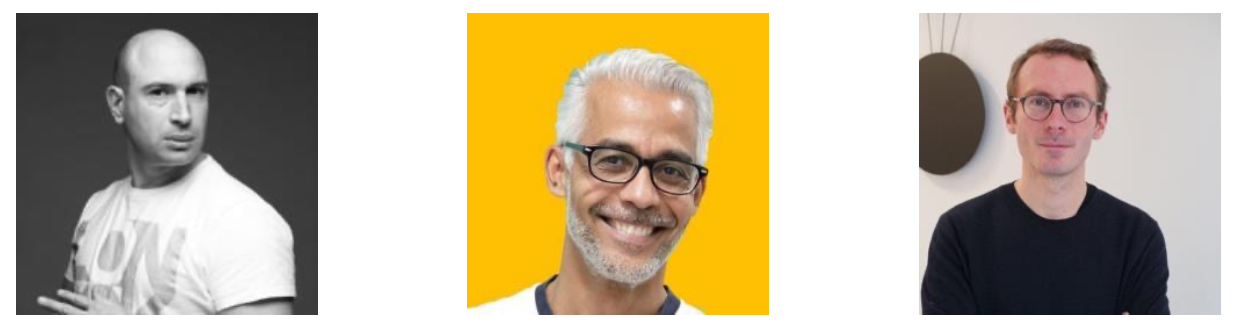
\includegraphics[width=0.8\textwidth]{Figures/direction}
	       \decoRule
		\caption[Direction]{Direction}
	\label{fig:Direction}
\end{figure}
M. Mickaël BENHASSEN est à la tête du département Tech dans lequel j’ai passé  mon stage. Ce département est celui qui dispose du plus grand nombre de recrues. J’ai pu travailler avec deux développeurs Pierre GANCEL, développeur front-end et Anderson LOYEM, développeur back-end, ainsi que quatre autres stagiaires comme moi :
Nikita KUMARI, Meriem BANOUNE, Josias SEMANOU et Ghaith MAGROUNE. Ensemble, nous avons réalisé les missions confiées en travaillant parfois à deux sur un sujet et j’ai pu bénéficier de l’aide de chacun d’eux durant mon expérience.\\ \\ Les autres départements sont celui des Opérations, chargé de la stratégie opérationnelle de l'entreprise et du développement de son activité, le Juridique et Finances qui veille au suivi des procédures juridiques et établit la stratégie financière, le Marketing et Communication qui élabore les plans marketing et s’occupe de la promotion de l’entreprise et enfin le département Commercial qui gère les ventes. Depuis peu, l’entreprise a embauché un responsable des Ressources Humaines, dont la mission sera de veiller au recrutement et à permettre la bonne santé et un environnement de travail sans stress à tous ses salariés.

 \begin{figure}[H]
            \centering
                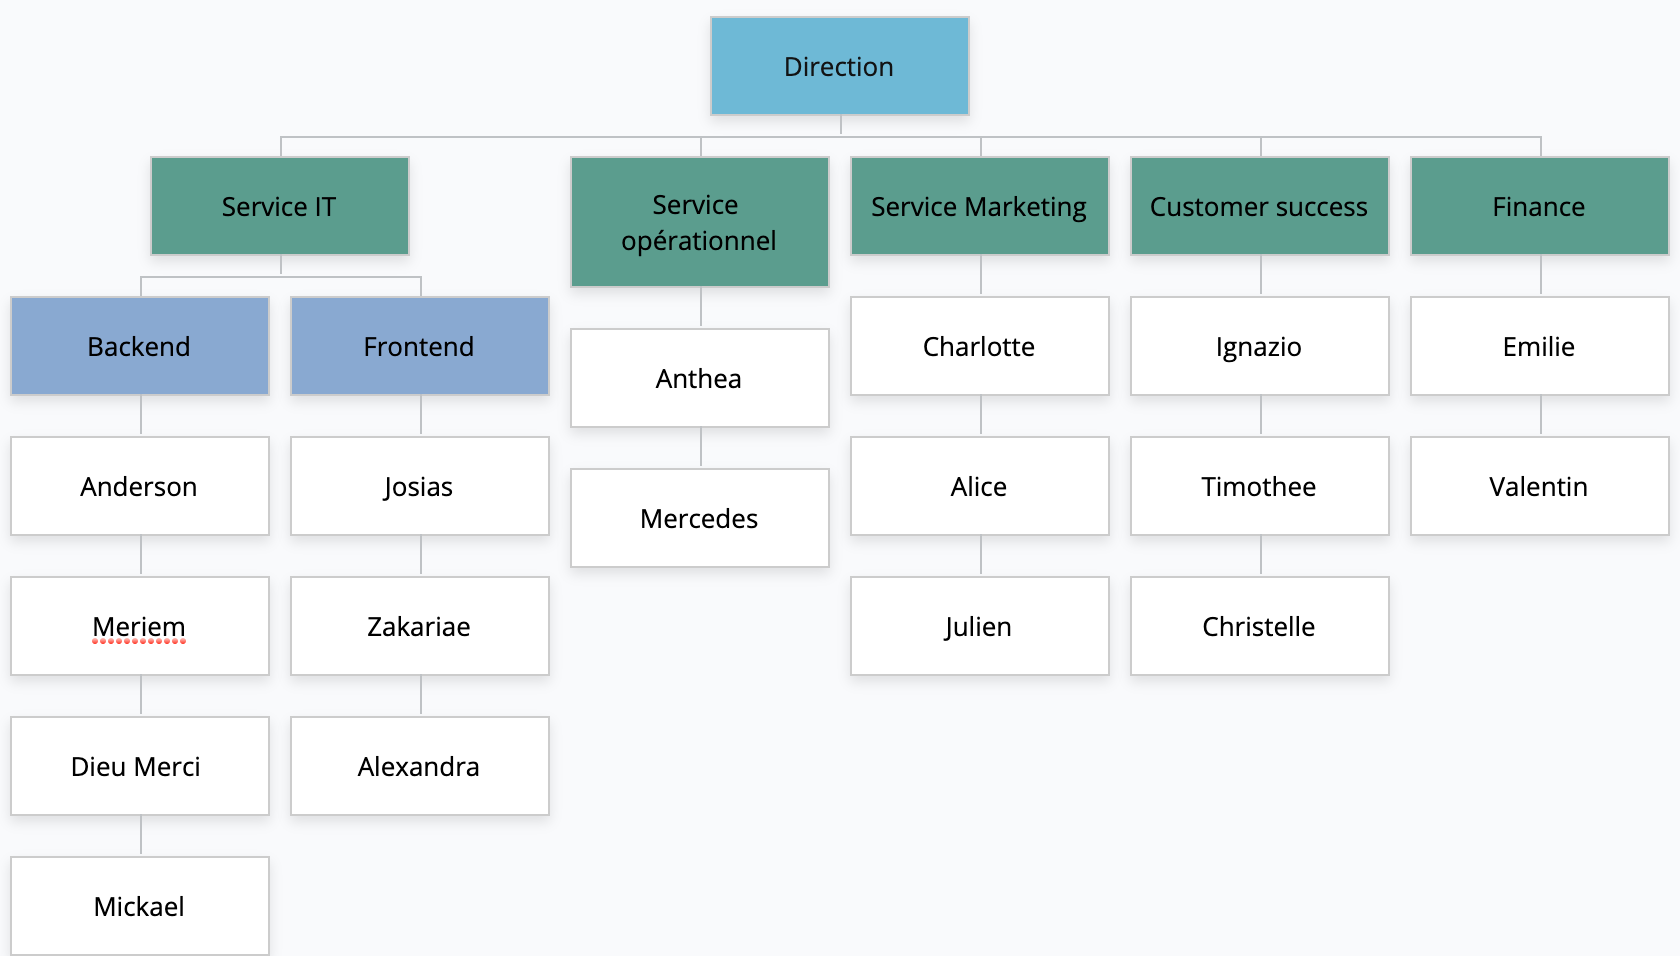
\includegraphics[width=0.8\textwidth]{Figures/orga}
	       \decoRule
		\caption[Organigramme]{Organigramme}
	\label{fig:Organigramme}
\end{figure}
 %\textbf{A compléter}
\newpage
\section{Localisation de Gigamesh :}

Localisé à Paris dans un espace de travail: \textbf{platform58}, \textbf{Gigamesh } profite d’un environnement de coworking et de bureaux privés. Un espace de coworking est un espace de travail partage mettant en avant l’échange et l’ouverture aux autres. Située au \textbf{58, rue de la Victoire 75009 Paris}, la \textbf{platform58} est un lieu d’innovation de la Banque Postale qui
repose sur deux briques :
\begin{itemize}
	\item Un programme d’accompagnement de startups
	\item Un lieu physique proposant la location d’espaces de travail
\end{itemize}

\section{Domaine d’activité de Gigamesh}
%Nous allons voir dans cette partie le domaine dans lequel évolue \textbf{Gigamesh} et la réponse apportée pour le faire progresser.
\subsection{Assurance emprunteur}

L’assurance de prêt généralement désignée par assurance emprunteur (article L. 313-29 du code de la
consommation) est une garantie demandée par les prêteurs (les banques) lors d’une demande de prêt.
Bien que ce ne soit pas une obligation légale, elle est exigée dans la quasi-totalité des cas. Cette assurance permet de couvrir les risques de défaut de paiement quelles que soient leurs causes, ce qui explique qu’elle soit ainsi exigée. Elle comporte des garanties couvrant les risques :
\begin{itemize}
	\item D’incapacité
	\item D’invalidité
	\item Voire de perte d’emploi
\end{itemize}

\begin{figure}[!th]
\centering
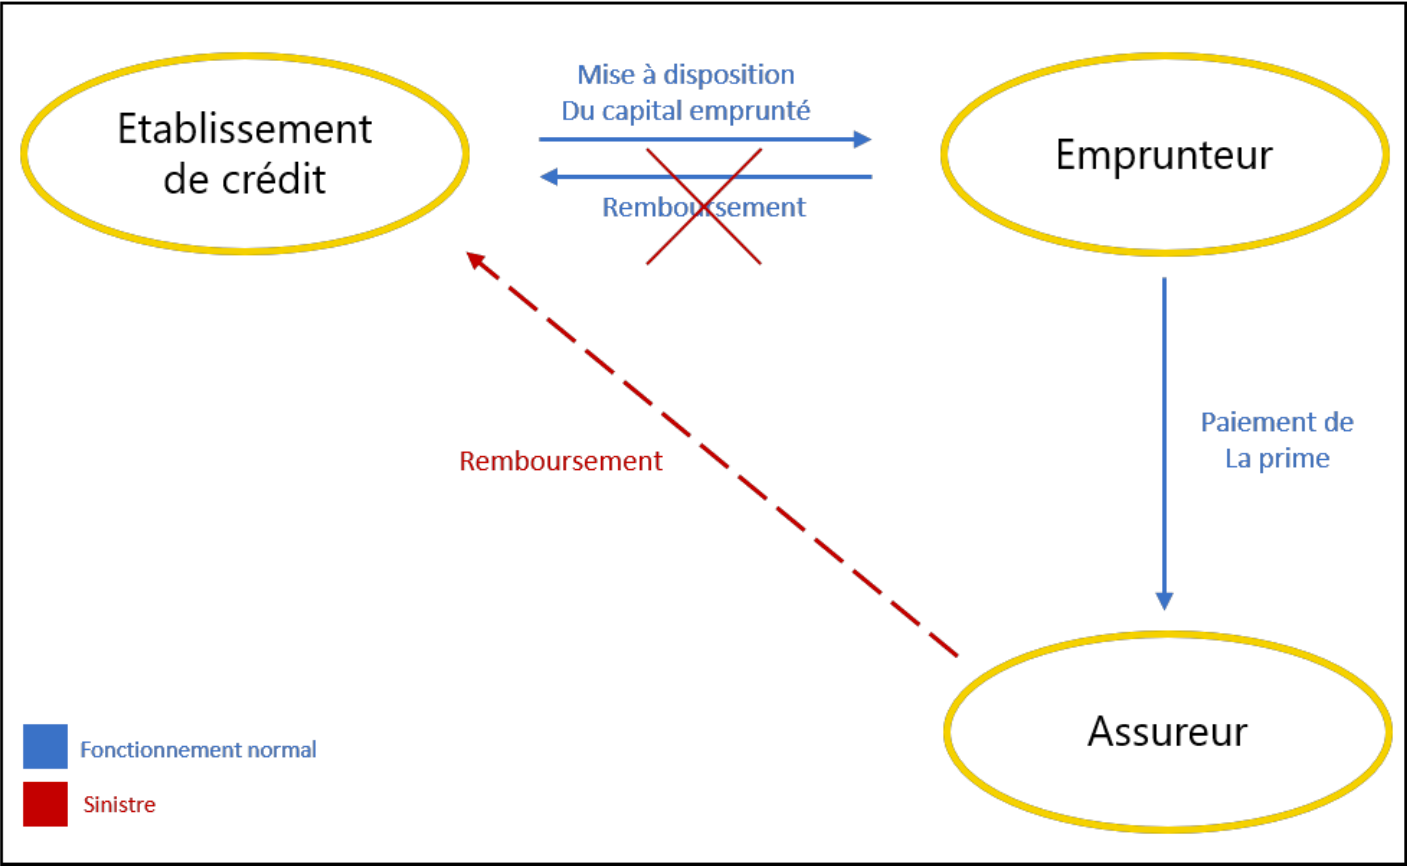
\includegraphics[width=0.8\textwidth]{Figures/emprunteur}
\decoRule
\caption[Illustration du système d'emprunt]{Illustration du système d'emprunt.}
\label{fig:Emprunt}
\end{figure}
\newpage
\subsection{Assurly}
Assurly est le nom donne au produit d’assurance de Gigamesh  et représente tout le travail effectue par l’entreprise depuis sa création. Assurly est donc le résultat du projet de Gigamesh. Assurly est une assurance emprunteur qui bouleverse le secteur de l’assurance en créant un produit clair, simple et au juste prix. \\ \\Tout est parti du constat que les assurances emprunteur traditionnelles ont construit leur analyse des risques sur une photographie figée de l’assuré, en décalage avec les nombreux changements que la vie réserve. Ils ont donc perdu de vue leur mission de départ : protéger en cas de problème.\\ \\ Suite à 3 ans de recherche et développement, Gigamesh a réussi à associer les apports de l’innovation technologique et leur expertise assurantielle pour créer Assurly.\\ \\Assurly est née avec l’ambition de redonner le pouvoir aux assurés en proposant un produit clair avec desgaranties all-inclusive au meilleur tarif. Assurly transforme l’assurance emprunteur grâce à une expérience client simplifiée et 100\% digitale : une souscription en moins de 10 minutes depuis son portable avec zéro paperasse, zéro rendez-vous, zéro stress !\\ \\Assurly propose de couvrir ces risques avec les garanties suivantes :

\begin{enumerate}
	\item La garantie perte totale et irréversible d’autonomie (PTIA).\\
	
Elle intervient lorsque l’assuré se trouve dans un état particulièrement grave, nécessitant le recours permanent à une tierce personne pour exercer les actes ordinaires de la vie.\\

\textbf{La couverture Assurly} : Gigamesh sera là pour vous épauler et rembourser 100\% des mensualités du reste de votre prêt. La garantie PTIA cesse au 71ème anniversaire de l’assuré.

\item La garantie incapacité temporaire totale (ITT) dénommée incapacité temporaire totale dans le contrat.\\ \\ Elle intervient lorsque la personne assurée est temporairement inapte à exercer son activité professionnelle ou, si il n’en a pas, d’observer un repos complet l’obligeant à interrompre toutes ses occupations de la vie
quotidienne\\
\textbf{La couverture Assurly} : Gigamesh sera là pour vous épauler et payer 100\% vos mensualités de remboursement de prêt durant votre temps d’impossibilité de travailler avec un plafond de 7500 euros par mois, quelle que soit votre perte de revenu. La garantie ITT cesse au plus tard au jour du 65ème anniversaire de l’assuré. Les affections dorsales, psychiques et psychiatriques causant l’ITT sont couvertes sans condition d’hospitalisation
ou d’intervention chirurgicale.
\begin{list}{label}{spacing}
	\item La garantie Invalidité prend deux formes :
	 \begin{enumerate}
	 	\item La garantie invalidité permanente partielle (IPP) :\\
	 	Elle intervient lorsque la personne assurée est, de façon définitive, incapable d’exercer strictement son
	 	activité après la reconnaissance de l’état d’invalidité estimé avec un taux entre 33\% et 66\%.\\
	 	
	 	\textbf{La couverture Assurly }: Gigamesh  sera là pour vous épauler et payer 50\% de l’indemnité garantie en cas d’ITT, quelle que soit votre perte de revenu, avec un plafond de 7500€ par mois. Le délai de franchise maximale est de 90 jours après l’interruption de l’activité. Les affections dorsales, psychiques et psychiatriques causant l’IPP sont couvertes sans condition d’hospitalisation
	 	ou d’intervention chirurgicale
	 	\item La garantie Invalidité Permanente Totale (I.P.T.)\\
	 	Elle intervient lorsque la personne assurée est, de
	 	façon définitive, incapable d’exercer strictement son activité professionnelle après la reconnaissance de l’état d’invalidité estimé avec un taux supérieur à 65\%\\
	 	
	 	\textbf{La couverture Assurly} : Gigamesh  sera là pour vous épauler et rembourser 100\% des mensualités du reste de votre prêt avec un plafond de 3 000 000 euros, quelle que soit votre perte de revenu. La garantie invalidité cesse au jour du 65ème anniversaire de l’assuré.
	 \end{enumerate}

\end{list}
\item La garantie décès\\
Elle intervient en cas de décès de la personne assurée. Nous serons là pour épauler votre famille et payer 100\% de vos mensualités de remboursement de votre prêt.

\end{enumerate}
\newpage
\section{Objectif du stage}
%Cette partie fera l’objet de la présentation du projet sur lequel j’avais travaillé et de mes propres mission dans ce celui ci:Assurly est une plateforme digitale et innovante, qui simplifie le système d’assurance d’emprunt. Elle est constituée des modules suivante:
Dans le cadre de son activité, le système d'Information de Gigamesh est constitué d’un frontend, d’un backend et d’applications tiers:
\begin{list}{•}
\item  Une application mobile B2C, pour la simulation de l’assurance et l’espace client,
\item
\item  Une application B2B, pour la simulation de l’assurance et de la création d’un assuré par des partenaires,
\item  Un ensemble d’application de gestion, paiement en ligne et service client,
\item Une application backend pour la gestion et données et la fourniture des APIs.
\end{list}  
Les applications frontend communiquent avec le backend via une API de type Rest.
Dans le cadre de mon stage j’intervenais plus souvent dans le backend et sur les missions suivantes:
\begin{list}{•}
	\item Le déploiement et l’intégration du service web (Reflex) dans un environnement AWS
	\item
	\item Intégration des données en format txt dans une base de données sql dans l’environnement AWS
	\item Etude de faisabilité sur le déploiement d’une application Front-End dans un environnement AWS
	\item Etude de la sécurité actuelle d’accès aux API.
	%\item Le déploiement d’un système de web scraping dans un environnement AWS.
\end{list}
\begin{figure}[H]
\centering
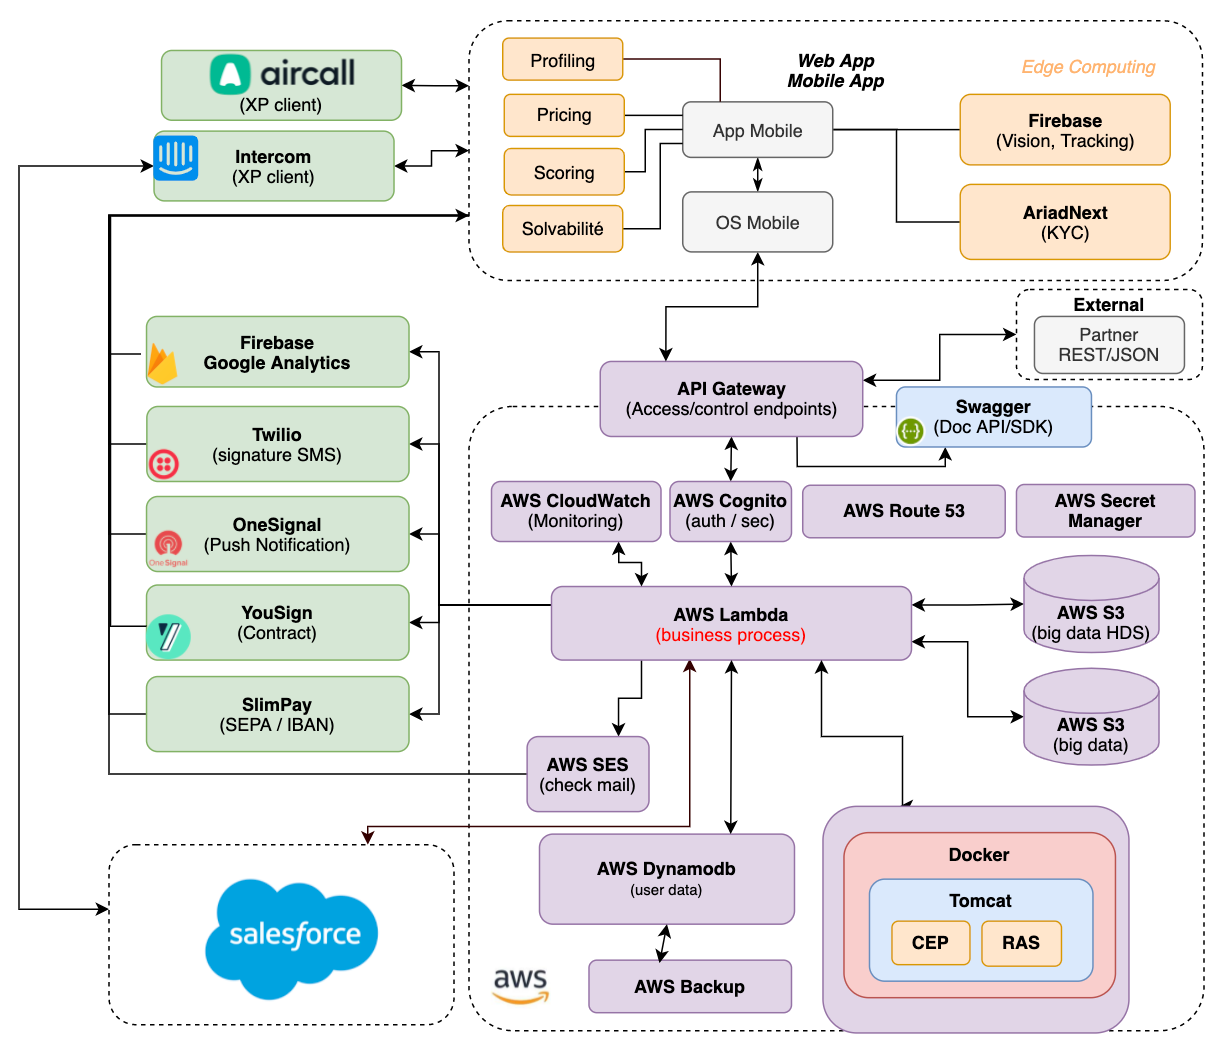
\includegraphics[width=0.8\textwidth]{Figures/architecture}
\decoRule
\caption[L'architecture globale du SI]{L'architecture globale du SI}
\label{fig:Architecture}
\end{figure}


%----------------------------------------------------------------------------------------




% Chaptre 1

\chapter{Etat de l’art} % Main chapter title

\label{Chaptre3} % For referencing the chapter elsewhere, use \ref{Chapter1} 

Dans cette partie nous présenterons le positionnement du travail demandé par rapport à l’état de l’art scientifique ou technique.

\section{Les APIs(Application programming interface)}

une API est une façade clairement délimitée par laquelle une application offre des services à d’autres applications. Cette façade peut comporter des classes, des méthodes ou des fonctions, des types de données et
des constantes. Les API peuvent être publiques, partenaires ou privées
 \begin{figure}[!th]
            \centering
                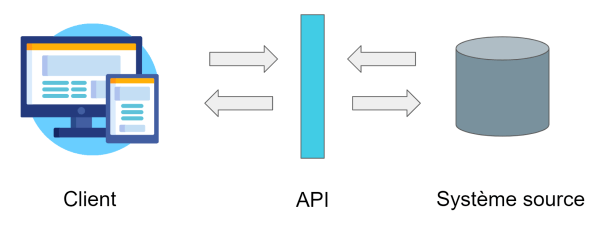
\includegraphics[width=0.8\textwidth]{Figures/api}
	       \decoRule
		\caption[API]{API}
	\label{fig:api}
	\end{figure}
\subsection{Objectif d’une API}
Tout comme une interface utilisateur graphique facilite l’utilisation des programmes pour les profanes, une
API a pour objectif de fournir une porte d’accès à une ou plusieurs fonctionnalités d’un système en exposant
uniquement les objets ou les actions dont le développeur a besoin et en cachant les détails de la mise en
œuvre. Elles permettent ainsi aux développeurs d’utiliser plus facilement certaines technologies pour créer
des applications. Une API simplifie la programmation.



\subsection{Analogie d’une API avec la vie courante}

Prenons l’exemple d’un appel téléphonique, la plupart des gens ne savent pas comment se déroule un appel
téléphonique : le mécanisme électronique qui régit un appel téléphonique. Pourtant tout le monde peut
effectuer un appel juste en composant le numéro de son correspondant et en appuyant simplement sur
un bouton (envoyer ou ok) du clavier. Le clavier et l’écran du téléphone sont l’équivalent de l’API; ils
représentent l’interface du système électronique qui régit un appel téléphonique

\section{Le modèle ou l'architecture Rest}
Les APIs peuvent être intégrées suivant plusieurs modèles ou styles d’architecture : le modèle à base des
simples fonctions, le modèle RPC, le modèle SOAP, le modèle Rest puis le modèle GraphQL.
Le modèle Rest, est un style orienté ressources et utilisant principalement le protocole HTTP pour la communication. Avec le modèle Rest les données entre le client et le fournisseur sont transmises en format JSON ou
XML. Ainsi, Rest utilise des notions qu’il faut obligatoirement comprendre : les ressources, les identifiants, les méthodes HTTP, et les formats de données.
\subsection{Les principes de l’architecture REST}
L'architecture Rest est régit par six principes suivants:
\begin{enumerate}
	\item La séparation entre client et serveur\\
les responsabilités du côté serveur et du côté client sont
séparées, si bien que chaque côté peut être implémenté indépendamment de l’autre. Le code
côté serveur (l’API) et celui côté client peuvent chacun être modifiés sans affecter l’autre, tant
que tous deux continuent de communiquer dans le même format. Dans une architecture REST,
différents clients envoient des requêtes sur les mêmes endpoints, effectuent les mêmes actions et
obtiennent les mêmes réponses.
     \item . L’absence d’état de sessions (stateless)\\
la communication entre client et serveur ne conserve pas
l’état des sessions d’une requête à l’autre. Autrement dit, l’état d’une session est inclus dans
chaque requête, ce qui signifie que ni le client ni le serveur n’a besoin de connaître l’état de
l’autre pour communiquer. Chaque requête est complète et se suffit à elle-même : pas besoin de maintenir une connexion continue entre client et serveur, ce qui implique une plus
grande tolérance à l’échec. De plus, cela permet aux APIs REST de répondre aux requêtes
de plusieurs clients différents sans saturer les ports du serveur. L’exception à cette règle est
l’authentification, pour que le client n’ait pas à préciser ses informations d’authentification à
chaque requête.
      \item L’uniformité de l’interface\\
les différentes actions et/ou ressources disponibles avec leurs endpoints et leurs paramètres spécifiques doivent être décidés et respectés religieusement, de façon
uniforme par le client et le serveur. Chaque réponse doit contenir suffisamment d’informations
pour être interprétée sans que le client n’ait besoin d’autres informations au préalable. Les
réponses ne doivent pas être trop longues et doivent contenir, si nécessaire, des liens vers d’autres
endpoints. 
       \item La mise en cache\\
les réponses peuvent être mises en cache pour éviter de surcharger inutilement le serveur. La mise en cache doit être bien gérée : l’API REST doit préciser si telle ou telle
réponse peut être mise en cache et pour combien de temps pour éviter que le client ne reçoive
des informations obsolètes.
        \item L’architecture en couches\\
un client connecté à une API REST ne peut en général pas distinguer
s’il est en communication avec le serveur final ou un serveur intermédiaire. Une architecture
REST permet par exemple de recevoir les requêtes sur un serveur A, de stocker ses données sur
un serveur B et de gérer les authentifications sur un serveur C.
        \item Le code à la demande
Cette contrainte est optionnelle. Elle signifie qu’une API peut retourner
du code exécutable au lieu d’une réponse en \textbf{JSON} ou en XML par exemple. Cela signifie qu’une
API \textbf{RESTful} peut étendre le code du client tout en lui simplifiant la vie en lui fournissant du
code exécutable tel qu’un script \textbf{JavaScript}.

\end{enumerate}

Une API REST ne peut être qualifiée de \textbf{RESTful} si elle ne respecte pas les six contraintes, mais on peut
tout de même la qualifier d’API REST si elle n’enfreint que deux ou trois principes. REST est sans doute le
standard le plus utilisé pour concevoir des architectures d’API, mais il en existe bien d’autres qui pourraient le complémenter, voire un jour le détrôner

\section{L’architecture serverless}
C’est une architecture où l’utilisateur n’a pas à gérer la moindre infrastructure. L’architecture serverless ne signifie pas pour autant qu’il n’y a pas de serveurs : cela veut dire qu’ils sont invisibles pour l’utilisateur et sont gérés par les fournisseurs et non par les consommateurs. Sans trop penser à leur maintenance, les ressources informatiques sont utilisées comme des services.
 
L’architecture serverless fait changer la façon dont on conçoit et maintient les applications. Elle permet aux consommateurs de bâtir des plateformes en utilisant exclusivement des services managés, de se concentrer sur les aspects liés à la logique business, et non sur les contraintes de déploiement ou de scalabilité.
\begin{list}{•}
	\item  Exemples fournisseur des architectures Serverless
	\begin{itemize}
		\item AWS
		\begin{list}{*}
			\item Amazon S3
			\item Amazon Dynamodb
			\item Amazon Lambda
        \end{list}
		\item Google:
		\begin{list}{*}
			\item Google Cloud Functions
		\end{list}
		\item Microsoft
		\begin{list}{*}
			\item Azure Functions
		\end{list}
	\end{itemize}

\end{list}


%----------------------------------------------------------------------------------------

\section{Le protocole OAuth2 et la délégation d’autorisation}

Le Oauth2 est la seconde version du protocole Oauth(Open Autorization). Connu comme protocole de
délégation d’autorisations, le Oauth2 est un protocole qui permet à une application d’obtenir une autorisation d’accès limitée aux ressources disponibles sur un serveur accessible via HTTP. Si ces ressources
n’appartiennent pas à l’application, l’autorisation d’accès lui est déléguée par le détenteur des ressources ;
au cas contraire l’application obtient l’autorisation en s’authentifiant avec ses identifiants. Avec le protocole Oauth2 le propriétaire de ressources ne partage pas ses identifiants avec l’application qui sollicite ses
ressources. Le protocole Oauth2 fournit un modèle dans lequel le détenteur de ressource peut accorder un
accès limité à ses données en émettant simplement un jeton temporaire, qui sera utilisé par cette application
sollicitant ses données pour s’identifier auprès du serveur de ressources. Le protocole Oauth2 met le propriétaire de ressources au cœur du système d’octroi d’autorisation. C’est le propriétaire de ressources qui
fait le lien entre ses comptes sur différentes applications sans que des administrateurs de la sécurité aient
besoin d’intervenir directement sur chaque application.

\subsection{Exemple d’implémentation du protocole Oauth2}

Le protocole Oauth2 est utilisé par plusieurs entreprises comme Facebook, Google et Twitter. L’exemple que nous proposons ici est celui qui permet
d’afficher instantanément les tweets sur Facebook sans avoir besoin de votre mot de passe Facebook

\subsection{Le vocabulaire du protocole Oauth2}
\textbf{Les rôles}: Le protocole Oauth2 identifie quatre rôles: Client, Propriétaire de ressources, Serveur d’autorisation
et Serveur de ressources.
\begin{list}{•}
	\item  Le détenteur des ressources(Resource Owner):\\
	 Le détenteur ou le propriétaire de ressources est
	une entité capable d’accorder l’accès à une ressource protégée. Lorsque le propriétaire de la ressource est une personne, on parle d’ utilisateur final.

	\item Le serveur de ressources (Resource Server):\\
	Le serveur de ressources est le serveur qui héberge
	les ressources protégées ou à accès limité. Un exemple du serveur des ressources peut être Facebook et Google qui hébergent les informations des profils des utilisateurs.
	\item Le client (Client Application): \\
	C’est une application qui sollicite les ressources du serveur de
	ressources, celle-ci peut être une application PHP, une application mobile, une application Javascrip.
	\item Le serveur d’autorisation (Authorization Server):\\
	Le serveur d’autorisation représente le serveur
	qui délivre des jetons au client. Ces jetons seront utilisés lors des requêtes du client vers le serveur de ressources. Ce serveur peut être le même que le serveur de ressources (physiquement et applicativement), et c’est souvent le cas.
\end{list}
\textbf{Les jetons:} Un jeton est une chaîne des caractères, générée par le serveur d’autorisation au client une fois
qu’ une autorisation lui est offerte.
\begin{list}{•}
	\item Le jeton d’accès(Access token):\\
	 est un jeton nécessaire pour accéder aux ressources partagées par
	OAuth2. Il a une durée de vie qui est généralement assez courte.
	\item  
	\item Le jeton de renouvellement (Refresh Token):\\
	 est un jeton que le serveur d’autorisation peut émettre aux clients et il peut être échangé contre un nouveau jeton d’accès, sans répéter le processus d’autorisation. Il n’a pas de temps d’expiration.
\end{list}

\textbf{Les types d’autorisations(Grant types)}

\begin{list}{•}
	\item L’autorisation implicite (Implicit Grant): \\
	Elle doit être utilisée quand l’application se trouve côté
	client(typiquement une application Javascript). Il ne permet pas d’obtenir de token de renouvellement.
	
	\begin{figure}[!th]
            \centering
                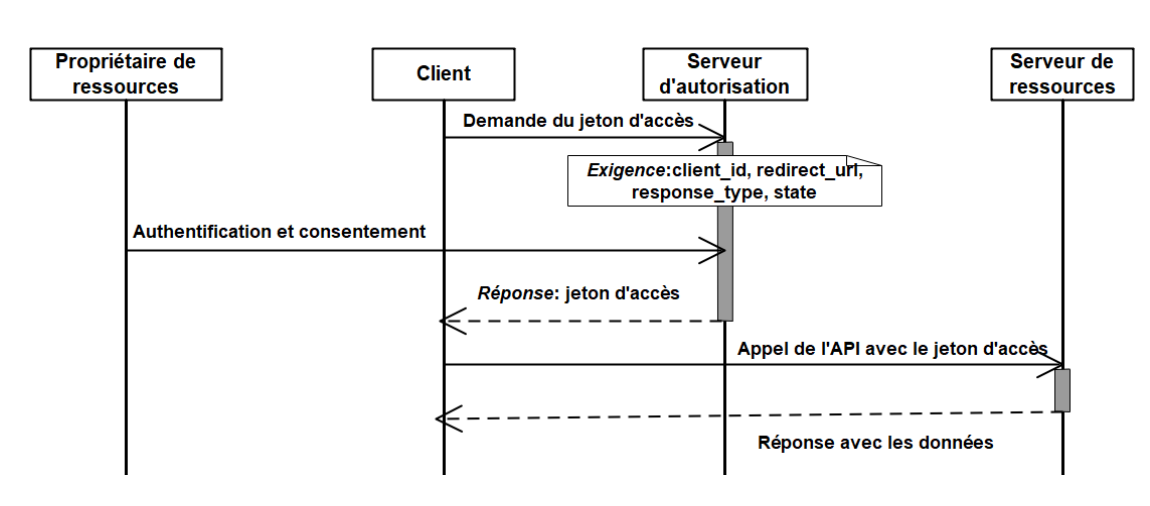
\includegraphics[width=0.8\textwidth]{Figures/implicit_grant}
	       \decoRule
		\caption[Implicit grant]{Implicit grant}
	\label{fig:implicit}
	\end{figure}
	
	\item L’autorisation via un code (Authorization Code Grant): \\
	Ce type d’autorisation permet d’obtenir deux jetons : le jeton d’accès et le jeton de renouvellement. Le client dans ce cas de figure interagit
	avec le propriétaire des ressources via un client web généralement un navigateur
	\begin{figure}[!th]
            \centering
                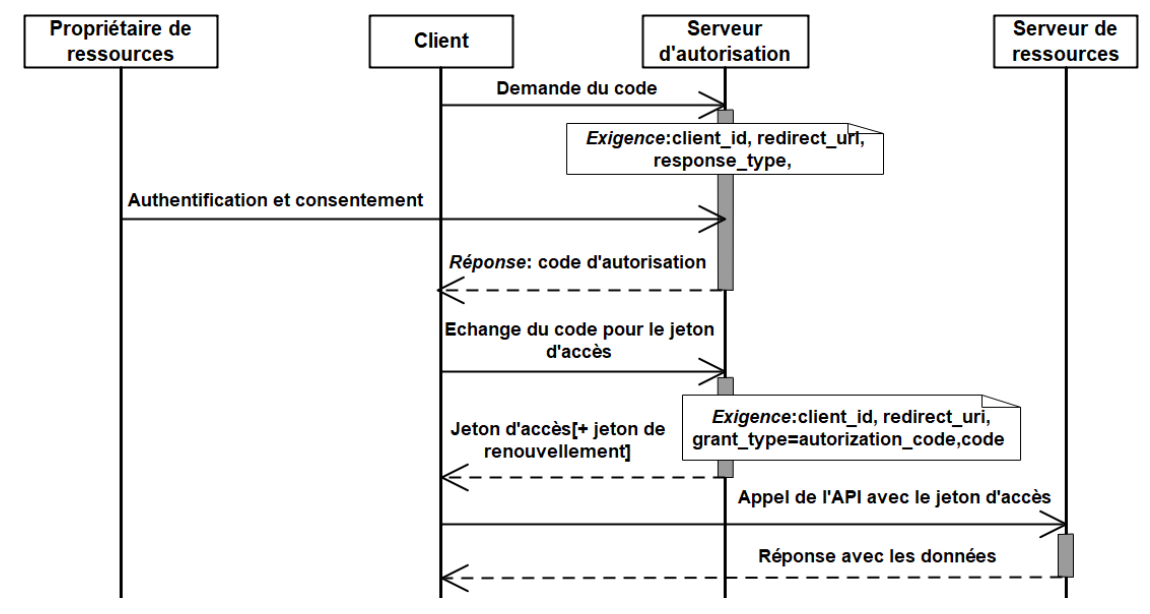
\includegraphics[width=0.8\textwidth]{Figures/code_grant}
	       \decoRule
		\caption[Code grant]{Code grant}
	\label{fig:Code}
	\end{figure}
	
	\item L’autorisation serveur à serveur (Client Credentials Grant):\\
	 Elle doit être utilisée lorsque le client est lui-même le détenteur des données. Il n’y a pas d’autorisation à obtenir de la part de l’utilisateur
	 \begin{figure}[!th]
            \centering
                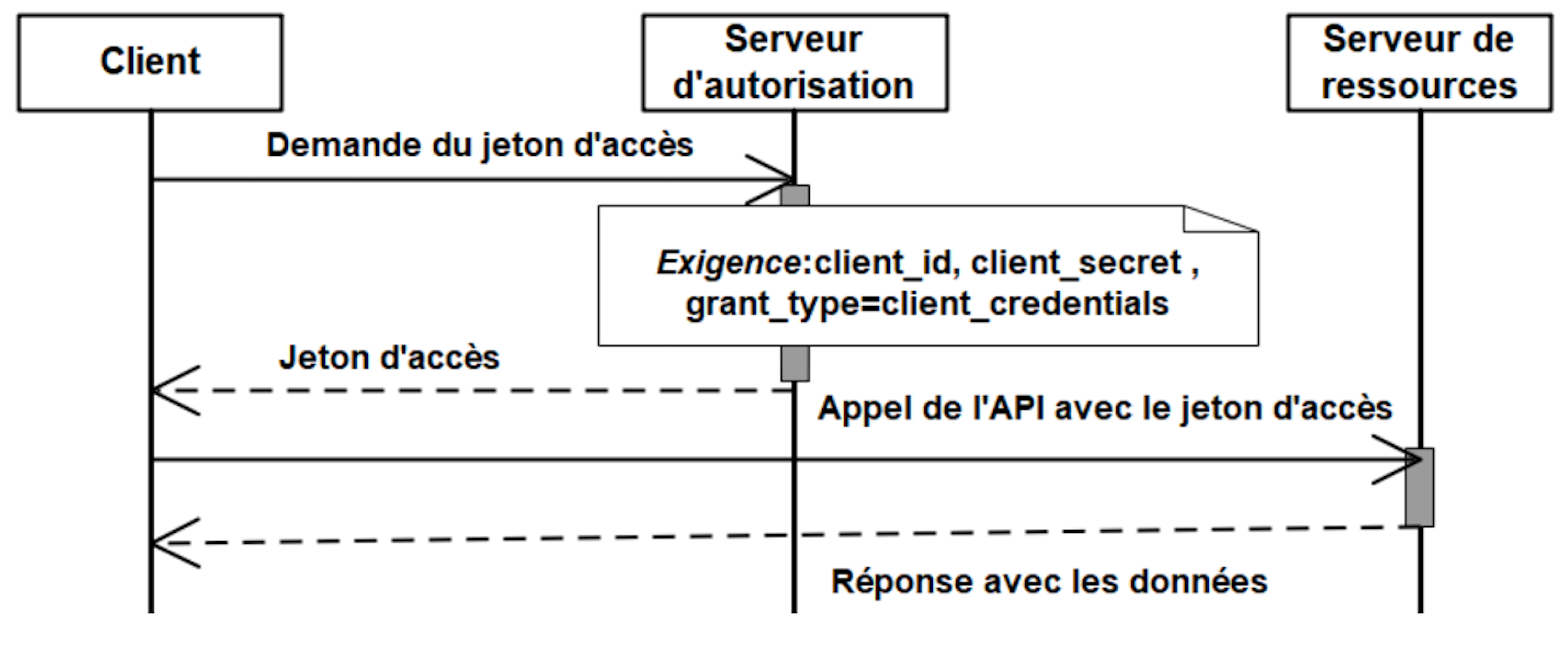
\includegraphics[width=0.8\textwidth]{Figures/server_server}
	       \decoRule
		\caption[Sever grant]{Server grant}
	\label{fig:Server}
	\end{figure}
	
	 \item L’autorisation via mot de passe (Resource Owner Password Credentials Grant):\\
	 Avec ce type d’autorisation, les identifiants sont envoyés au client et ensuite au serveur d’autorisation. Il est donc
	 impératif qu’il y ait une confiance absolue entre ces 2 entités. Ce type d’autorisation est principalement utilisé lorsque le client a été développé par la même autorité que celle          fournissant le serveur d’autorisation final.
	 \begin{figure}[!th]
            \centering
                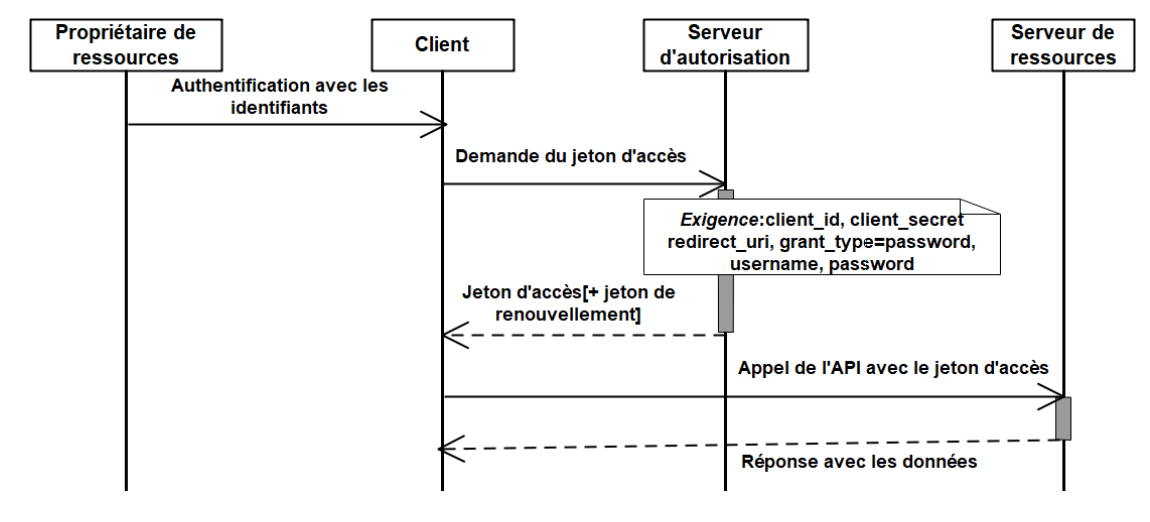
\includegraphics[width=0.8\textwidth]{Figures/password_grant}
	       \decoRule
		\caption[Password grant]{Password grant}
	\label{fig:Password}
	\end{figure}
\end{list}


%----------------------------------------------------------------------------------------
\section{Intégration de données}
L’intégration des données est le processus qui consiste à combiner des données provenant de différentes
sources dans une vue unifiée : de l’importation au nettoyage en passant par le mapping et la transformation dans un gisement cible, pour finalement rendre les données plus exploitables et plus utiles pour les
utilisateurs qui les consultent.
\subsection{Les avantages}
\begin{list}{•}
	\item L’intégration des données améliore l’unification des systèmes et la collaboration globale
	\item L’intégration des données fait gagner du temps
	\item L’intégration des données réduit les erreurs (et les besoins de modifications)
\end{list}
\subsection{Opérations ETL et intégration des données}
Les opérations d’extraction, de transformation et de chargement (ETL) forment un processus d’intégration
à part entière dans lequel les données sont extraites du système source et livrées au data warehouse. Il s’agit
d’un processus continu que le data warehousing exécute pour transformer plusieurs sources de données en
informations cohérentes et utiles destinées à la Business Intelligence et aux analyses.
 \begin{figure}[!th]
            \centering
                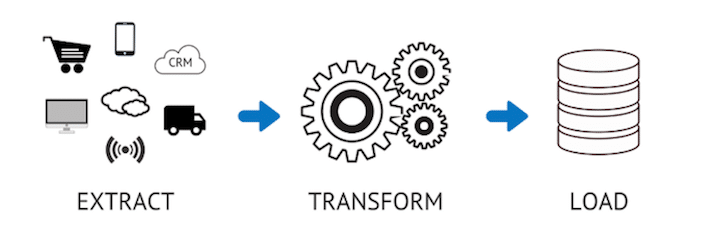
\includegraphics[width=0.8\textwidth]{Figures/etl}
	       \decoRule
		\caption[ETL]{ETL}
	\label{fig:ETL}
	\end{figure}
\section{Conteneurisation}
Un conteneur est un système qui permet de stocker et d’isoler des objets devant être transportés ou déployés dans un environnement d’exploitation étendu (applications, logiciels, librairie, etc.). Il permet également au code applicatif d’être transporté de l’environnement de développement vers celui de production de manière aisée et sûre.  
La conteneurisation permet:
%La conteneurisation permet 

\begin{list}{•}
	\item De virtualiser, à l’intérieur d’un conteneur les ressources matérielles dont une application a besoin pour être exécutée(mémoire, réseau, processeur, etc.) 
	\item
	\item D'embarquer les composants logiciels nécessaires à l’application (données, fichiers, etc.)  
\end{list}

La conteneurisation est parfois confondue avec la virtualisation. Quand la première nécessite que chaque machine virtuelle possède 
son système d’exploitation, les conteneurs eux se connectent au noyau des machines, kernel, pour en exploiter les ressources. 
Moins lourds, ils sont plus faciles à déplacer et à stocker. 
 \begin{figure}[!th]
            \centering
                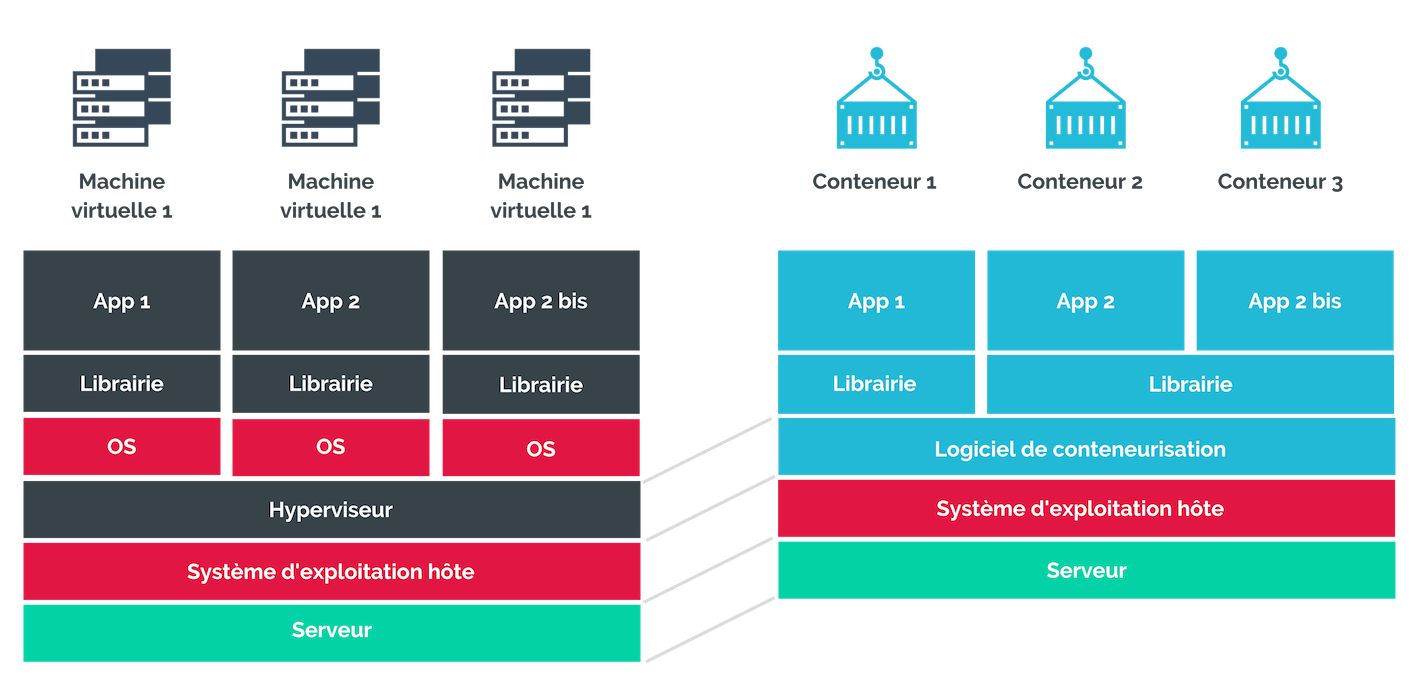
\includegraphics[width=0.8\textwidth]{Figures/virtualvscont}
	       \decoRule
		\caption[VM vs Conteneurisation]{VM vs Conteneurisation}
   \label{fig:VM vs Conteneurisation}
\end{figure}
%link : https://codalis.ch/conteneurisation-docker/

%Il s’agit d’un type de virtualisation utilisé au niveau des applications. Le principe repose sur la création de
%plusieurs espaces utilisateurs isolés les uns des autres sur un noyau commun. On utilise alors le terme de
%« conteneur » pour désigner une telle instance. Cette séparation repose sur un concept similaire à celui des
%modules applicatifs cloisonnés, communiquant à l’aide de services et applications web. Les conteneurs,
%bien qu’ indépendants, partagent un noyau commun (donc un ou plusieurs systèmes d’exploitation) et un
%même espace mémoire.
%La conteneurisation permet de packager tous les services, scripts, API, librairies dont une application a
%besoin. L’objectif : en permettre l’exécution sur n’importe quel noyau compatible
\subsection{Avantages}
\begin{list}{•}
	\item Elle évite de se soucier d’interactions ou d’incompatibilités avec les conteneurs déjà présents ou à
	venir sur cette machine.
	\item 
	\item Elle permet de ne pas occuper autant de ressources que réclamerait une machine virtuelle (ou virtual machine, VM), qui emporte son propre système d’exploitation et bloque des ressources à son
	lancement.
\end{list}
\subsection{Exemple des systèmes de conteneurisation}
\begin{list}{•}
	\item Docker
	\item Kubernetes
	\item CoreOs rkt
	\item OpenV
\end{list}
 
% Chaptre 1

\chapter{Outils et technologies utilisés} % Main chapter title

\label{Chaptre3} % For referencing the chapter elsewhere, use \ref{Chapter1} 

Dans cette section je vais présenter les outils et les technologies que j’avais utilisé durant mon stage.

%----------------------------------------------------------------------------------------

% Define some commands to keep the formatting separated from the content 
%\newcommand{\keyword}[1]{\textbf{#1}}
%\newcommand{\tabhead}[1]{\textbf{#1}}
%\newcommand{\code}[1]{\texttt{#1}}
%\newcommand{\file}[1]{\texttt{\bfseries#1}}
%\newcommand{\option}[1]{\texttt{\itshape#1}}
%----------------------------------------------------------------------------------------

\section{Amazon Lambda}
AWS Lambda est un service de calcul Serverless qui vous permet d’exécuter du code sans:
\begin{list}{•}
	\item provisionner ou gérer des serveurs,
	\item créer une logique de dimensionnement de cluster prenant en charge la charge de travail,
	\item  maintenir les intégrations d’événements ou gérer les environnements d’exécution.
\end{list}
Avec Lambda, vous pouvez exécuter du code pour pratiquement n’importe quel type d’application ou service backend , sans aucune tâche administrative. Il suffit de télécharger votre code sous forme de fichier
ZIP ou d’image de conteneur, et Lambda alloue automatiquement et précisément la puissance d’exécution
de calcul et exécute votre code en fonction de la demande ou de l’événement entrant, pour n’importe quelle
échelle de trafic.
Vous pouvez configurer votre code de sorte qu’il se déclenche automatiquement depuis plus de 200 applications SaaS et services AWS, ou l’appeler directement à partir de n’importe quelle application web ou
mobile.
Vous pouvez écrire des fonctions Lambda dans votre langage préféré (Node.js, Python, Go, Java, etc.)
\subsection{Fonctionnement}
Chaque fonction Lambda s'exécute dans son propre conteneur. Lorsqu'une fonction est créée, Lambda l'empaquette dans un nouveau conteneur, puis exécute ce conteneur sur un cluster de machines mutualisées géré par AWS. Avant que les fonctions ne commencent à s'exécuter, le conteneur de chaque fonction se voit allouer la mémoire RAM et la capacité CPU nécessaires. Une fois que les fonctions ont fini de s'exécuter, la RAM allouée au début est multipliée par le temps que la fonction a passé à s'exécuter. Les clients sont ensuite facturés en fonction de la mémoire allouée et de la durée d'exécution de la fonction.
\subsection{Avantages}
\begin{list}{•}
	\item Aucun serveur à gérer:
	AWS Lambda exécute automatiquement votre code, sans que vous ayez à mettre en service ou à gérer des
	serveurs
	\item Dimensionnement continu:
	AWS Lambda dimensionne automatiquement votre application en exécutant le code en réponse à chaque
	déclencheur. Votre code s’exécute en parallèle et traite chaque déclencheur indépendamment. La charge de
	travail est ainsi mise à l’échelle de façon précis
	\item Optimisation des coûts grâce au comptage en millisecondes:
	Avec AWS Lambda, vous ne payez que pour le temps de calcul que vous consommez
	\item Performances constantes à n’importe quelle échelle:
	Avec AWS Lambda, vous pouvez optimiser le temps d’exécution de votre code en choisissant la bonne taille de mémoire pour
	votre fonction
\end{list}

%----------------------------------------------------------------------------------------

\section{Docker}
Docker est un système de containérisation le plus utilisé; qui vous permet de créer, déployer et lancer vos applications en utilisant des conteneurs.
Pour mettre en place ces conteneurs, on crée des images Docker. L’image Docker permet de configurer tout l’environnement dans lequel le conteneur va s'exécuter. 
Pour créer ces images, Docker utilise un fichier spécial appelé Dockerfile, qui grâce à une syntaxe simple et élégante va nous permettre de préparer nos images.
L’image est ensuite construite par le démon Docker via l’utilisation de commandes dans le terminal qui sont regroupées dans ce qu’on appelle un CLI.
Pour gérer l’ensemble des conteneurs d’une application, on utilise Docker Compose.

 \begin{figure}[H]
            \centering
                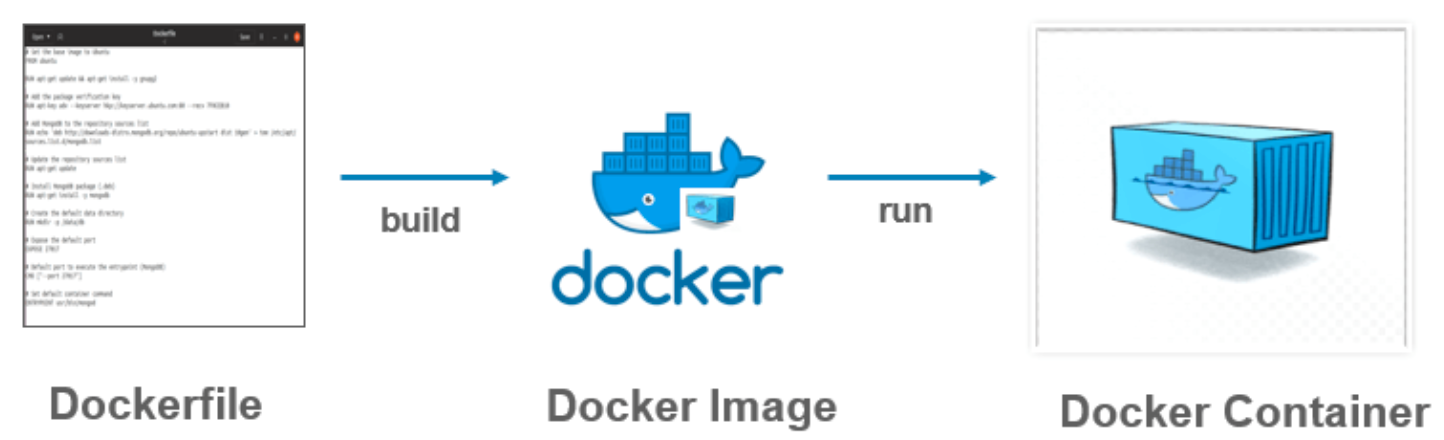
\includegraphics[width=0.8\textwidth]{Figures/dockerfileimagecontainer}
	       \decoRule
		\caption[Docker]{Docker}
	\label{fig:docker}
\end{figure}
Un conteneur est une instance d'une image et une image est obtenue on compilant le fichier Dockerfile.
\subsection{Docker Hub}
Docker Hub est un service fourni par Docker pour rechercher et partager des images de conteneurs avec votre équipe. 
Il s'agit du plus grand référentiel au monde d'images de conteneurs.
Docker Hub fournit les fonctionnalités principales suivantes :
\begin{list}{•}
	\item Repositories: permet le push et le pull des images des conteneurs
	\item Teams and  Organizations: permet de gérer l'accès aux référentiels privés d'images de conteneurs
	\item Docker Official Images: permet de récupéré  et d'utiliser des images de conteneurs de haute qualité fournies par Docker
	\item Builds: permet de créer automatiquement des images de conteneur à partir de GitHub et Bitbucket et de les transférer vers Docker Hub.
\end{list}
Docker fournit un outil  Docker Hub CLI  et une API qui vous permet d'interagir avec Docker Hub.


\section{Amplify}

AWS Amplify est un ensemble d’outils et de services qui peuvent être utilisés ensemble ou un par un, pour:
\begin{list}{•}
\item Authentification: accéder à des workflows prêts à l'emploi pour MFA, authentification unique, mot de passe oublié, etc.
\item Hébergement: déployer des applications Web statiques en quelques clics et facilement gérer le contenu(JavaScript, React, Angular, Flutter,...)
\item Notifications push: gérer facilement les campagnes et envoyer des messages aux utilisateurs via plusieurs canaux, notamment par SMS, e-mail et push.
\item Analytique: suivre les sessions des utilisateurs et créer des rapports sur leur comportement. Configurer des attributs personnalisés et analyser les entonnoirs de conversion.
\end{list}

%link : https://www.bluematador.com/blog/what-is-aws-amplify
%aider les développeurs web mobile et frontal à créer des applications évolutives et intégrales à technologie
%AWS. Avec Amplify, vous pouvez configurer les backends d’application et connecter votre application en
%quelques minutes, déployer des applications Web statiques en quelques clics et facilement gérer le contenu
%des applications en dehors de la console AWS.
%Amplify prend en charge les frameworks Web populaires, tels que JavaScript, React, Angular, Vue, Next.js,
%et les plateformes mobiles, telles qu’Android, iOS, React Native, Ionic, Flutter.
%\subsubsection{Developpement}
 \begin{figure}[H]
            \centering
                \includegraphics[width=0.8\textwidth]{Figures/amplify_dif}
	       \decoRule
		\caption[Exemple d'hébergement d'un site static]{Exemple d'hébergement d'un static}
	\label{fig:amplify}
	\end{figure}
%\subsubsection{}
% \begin{figure}[H]
%            \centering
%              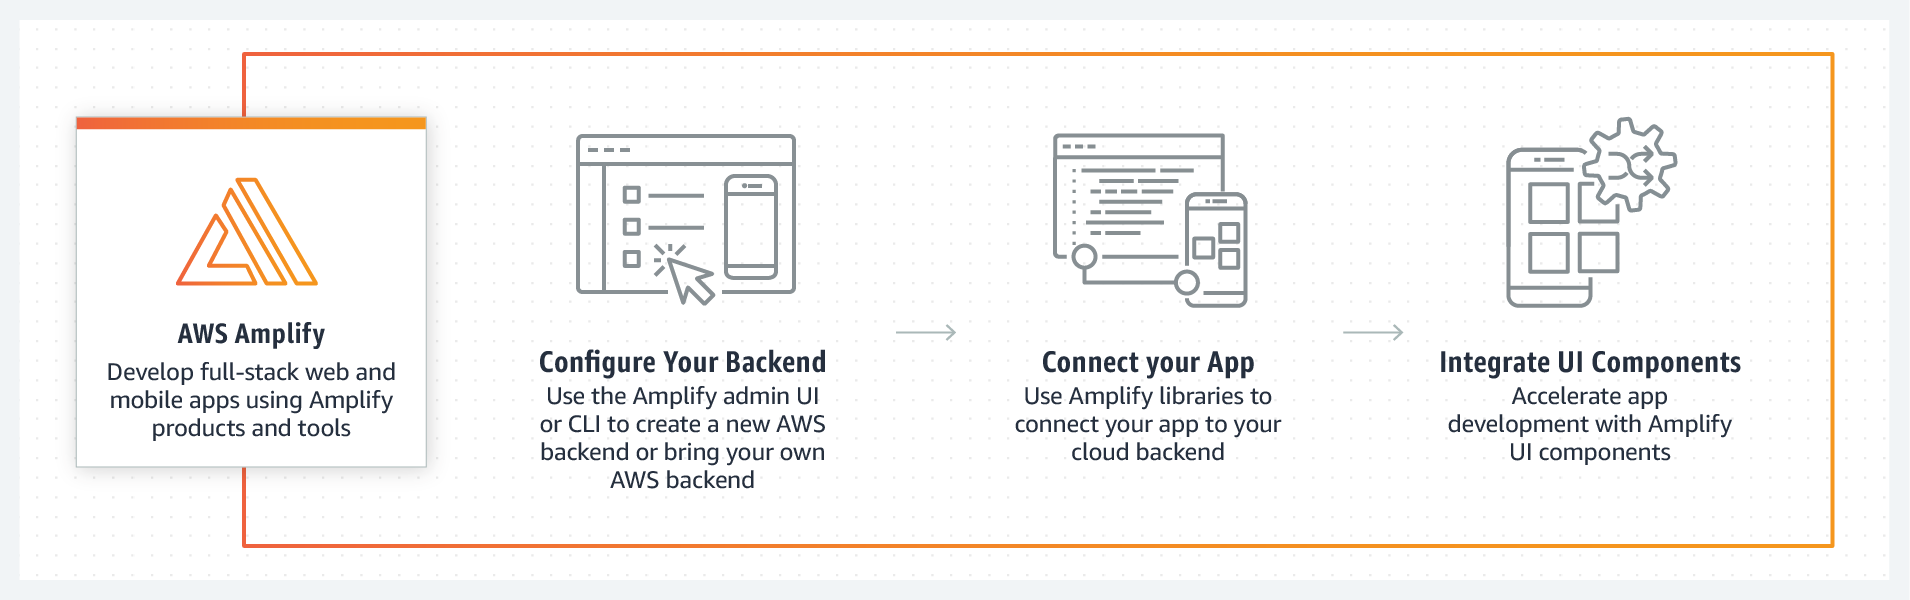
\includegraphics[width=0.8\textwidth]{Figures/amplify-2}
%	       \decoRule
%		\caption[Amplify]{Amplify}
%	\label{fig:amplify}
%	\end{figure}

\section{Amazon Simple Storage Service (Amazon S3)}
Amazon S3 est un stockage d'objets conçu pour stocker et récupérer n'importe quelle quantité de données, n'importe où. Il s'agit d'un service de stockage simple qui offre une durabilité, une disponibilité, des performances, une sécurité, et une scalabilité de pointe pratiquement illimitée à un tarif très bas.
S3 supporte tout type de fichier et peut être utilisé comme repos d'hébergement des sites web statics:
\subsection{Avantages de l'utilisation d'Amazon S3}
Amazon S3 est intentionnellement conçu avec un ensemble de fonctionnalités minimal qui met l'accent sur la simplicité et la robustesse. Voici quelques-uns des avantages de l'utilisation d'Amazon S3 :
\begin{list}{•}
\item \textbf{Création de compartiments:}Créez et nommez un compartiment qui stocke les données. Les compartiments sont les conteneurs fondamentaux d'Amazon S3 pour le stockage de données.
\item \textbf{Stockage de données:}Stockez une quantité infinie de données dans un bucket. Chargez autant d'objets que vous le souhaitez dans un compartiment Amazon S3. Chaque objet peut contenir jusqu'à 5 To de données. Chaque objet est stocké et récupéré à l'aide d'une clé unique attribuée par le développeur.
\item \textbf{Téléchargement de données:}Téléchargez vos données ou permettez à d'autres de le faire. Téléchargez vos données à tout moment ou permettez à d'autres de faire de même.
\item \textbf{Autorisations:}Accordez ou refusez l'accès à d'autres personnes qui souhaitent charger ou télécharger des données dans votre compartiment Amazon S3. Accordez des autorisations de chargement et de téléchargement à trois types d'utilisateurs. Les mécanismes d'authentification peuvent aider à protéger les données contre les accès non autorisés.
\item \textbf{Interfaces standard:}Utilisez des interfaces REST et SOAP basées sur des normes conçues pour fonctionner avec n'importe quelle boîte à outils de développement Internet.
\end{list}


%S3 est un service de stockage d’objet offrant une évolutivité, une disponibilité des données, une sécurité et des performances de pointe. Les clients de toutes tailles et de tous secteurs peuvent ainsi utiliser
%ce service afin de stocker et protéger n’importe quelle quantité de données pour un large éventail de cas
%d’utilisation comme des lacs de données, des sites web, des applications mobiles, la sauvegarde et la restauration, l’archivage, des applications d’entreprise, des appareils IoT et des analyses du Big Data. Amazon
%S3 fournit des fonctions de gestion faciles à utiliser pour vous permettre d’organiser vos données et de
%configurer des contrôles d’accès affinés pour vos exigences métier, d’organisation et de conformité spécifiques. Amazon S3 est conçu pour offrir 99,999999999 \% de durabilité et stocker les données de millions
%d’applications pour des entreprises du monde entier

\section{Aws Aurora}

Amazon Aurora est un moteur de base de données relationnelle qui associe la vitesse et la fiabilité des bases
de données commerciales haut de gamme à la simplicité et la rentabilité des bases de données open source.
Amazon Aurora MySQL offre des performances jusqu’à cinq fois supérieures à celles de MySQL sans
nécessiter de modifications de la plupart des applications MySQL. De la même manière, Amazon Aurora
PostgreSQL offre des performances jusqu’à trois fois supérieures à celles de PostgreSQL. Amazon RDS
gère vos bases de données Amazon Aurora en prenant en charge les tâches chronophages telles que la mise en service, l’application des correctifs, la sauvegarde, la récupération, la détection des pannes, ainsi que
les réparations. Vous payez un forfait mensuel pour chaque instance de base de données Amazon Aurora
utilisée. Aucun coût initial ou engagement à long terme n’est requis.

\subsection{Que signifie « des performances trois fois supérieures à celles de PostgreSQL  et MySQL» }
Amazon Aurora fournit des augmentations significatives des performances de PostgreSQL et  MySQL en intégrant étroitement au moteur de base de données une couche de stockage virtualisée basée sur SSD, conçue principalement pour les charges de travail des bases de données, ce qui permet de réduire les opérations d'écritures dans le système de stockage, minimiser la contention de verrouillage et éliminer les retards créés par les threads de processus de la base de données

\section{Amazon Cognito}
Amazon Cognito permet d’ajouter facilement et rapidement l’inscription et la connexion des utilisateurs ainsi que le contrôle d’accès aux applications Web et mobiles. Amazon Cognito s’adapte à des millions d’utilisateurs et prend en charge la connexion avec les fournisseurs d’identité sociale tels qu’Apple, Facebook, Google et Amazon.\\ Amazon Cognito prend en charge les normes de gestion des identités et des accès, telle que Oauth 2.0.
%, et les fournisseurs d’identité d’entreprise via SAML 2.0 et OpenID Connect

%\subsection{Fonctionnalités}
%\subsubsection{Répertoire d’utilisateurs sécuritaire et se mettant à l’échelle}Les groupes d’utilisateurs d’Amazon Cognito fournissent un répertoire d’utilisateurs sécurisé qui s’étend à
%des centaines de millions d’utilisateurs. En tant que service entièrement géré, les groupes d’utilisateurs sontfaciles à configurer sans avoir à s’inquiéter de la mise en place d’une infrastructure serveur.
%\subsubsection{Fédération d’identité sociale et d’entreprise}
%Avec Amazon Cognito, vos utilisateurs peuvent se connecter via des fournisseurs d’identité sociale tels
%que Apple, Google, Facebook et Amazon.

%\subsubsection{Authentification basée sur les standards}
%Amazon Cognito User Pools est un fournisseur d’identités normalisé et prend en charge les normes degestion des identités et des accès, telle que Oauth 2.0.
%\subsubsection{Sécurité pour vos applications et vos utilisateurs}
%Amazon Cognito prend en charge l’authentification multi-facteurs et le chiffrement des données au repos et
%en transit. Amazon Cognito est éligible HIPAA et conforme aux normes PCI DSS, SOC, ISO/IEC 27001,ISO/IEC 27017, ISO/IEC 27018, et ISO 9001.
%\subsubsection{Contrôle d’accès pour les ressources AWS}Amazon Cognito fournit des solutions pour contrôler l’accès aux ressources AWS à partir de votre application. Vous pouvez définir des rôles et associer des utilisateurs à des rôles différents afin que votre
%application puisse accéder uniquement aux ressources autorisées pour chaque utilisateur. Autre possibilité: vous pouvez également utiliser les attributs des fournisseurs d’identité dans les stratégies d’autorisationAWS Identity and Access Management. Cela vous permettra de contrôler l’accès à des ressources pour lesutilisateurs qui remplissent des conditions d’attributs spécifiques
%\subsubsection{Intégration facile avec votre application}Amazon Cognito fournit des solutions pour contrôler l’accès aux ressources AWS à partir de votre application. Vous pouvez définir des rôles et associer des utilisateurs à des rôles différents afin que votreapplication puisse accéder uniquement aux ressources autorisées pour chaque utilisateur. Autre possibilité: vous pouvez également utiliser les attributs des fournisseurs d’identité dans les stratégies d’autorisationAWS Identity and Access Management. Cela vous permettra de contrôler l’accès à des ressources pour lesutilisateurs qui remplissent des conditions d’attributs spécifiques.


\section{API Gateway}

Amazon API Gateway est un service entièrement opéré, qui permet aux développeurs de créer, publier,
gérer, surveiller et sécuriser facilement des API à n’importe quelle échelle. Les API servent de « porte
d’entrée » pour que les applications puissent accéder aux données, à la logique métier ou aux fonctionnalités de vos services backend. À l’aide d’API Gateway, vous pouvez créer des API RESTful et des API
WebSocket qui permettent de concevoir des applications de communication bidirectionnelle en temps réel.
API Gateway prend en charge les charges de travail conteneurisées et sans serveur, ainsi que les applications
web.\\
API Gateway gère toutes les tâches liées à l’acceptation et au traitement de plusieurs centaines de milliers
d’appels d’API simultanés, notamment la gestion du trafic, la prise en charge de CORS, le contrôle des
autorisations et des accès, la limitation, la surveillance et la gestion de la version de l’API. Aucuns frais
minimum ou coûts initiaux ne s’appliquent à API Gateway. Vous payez pour les appels d’API que vous
recevez et la quantité de données transférées et, avec le modèle de tarification par paliers de l’API Gateway,
vous pouvez réduire vos coûts en fonction de l’utilisation de votre API

 \begin{figure}[H]
            \centering
                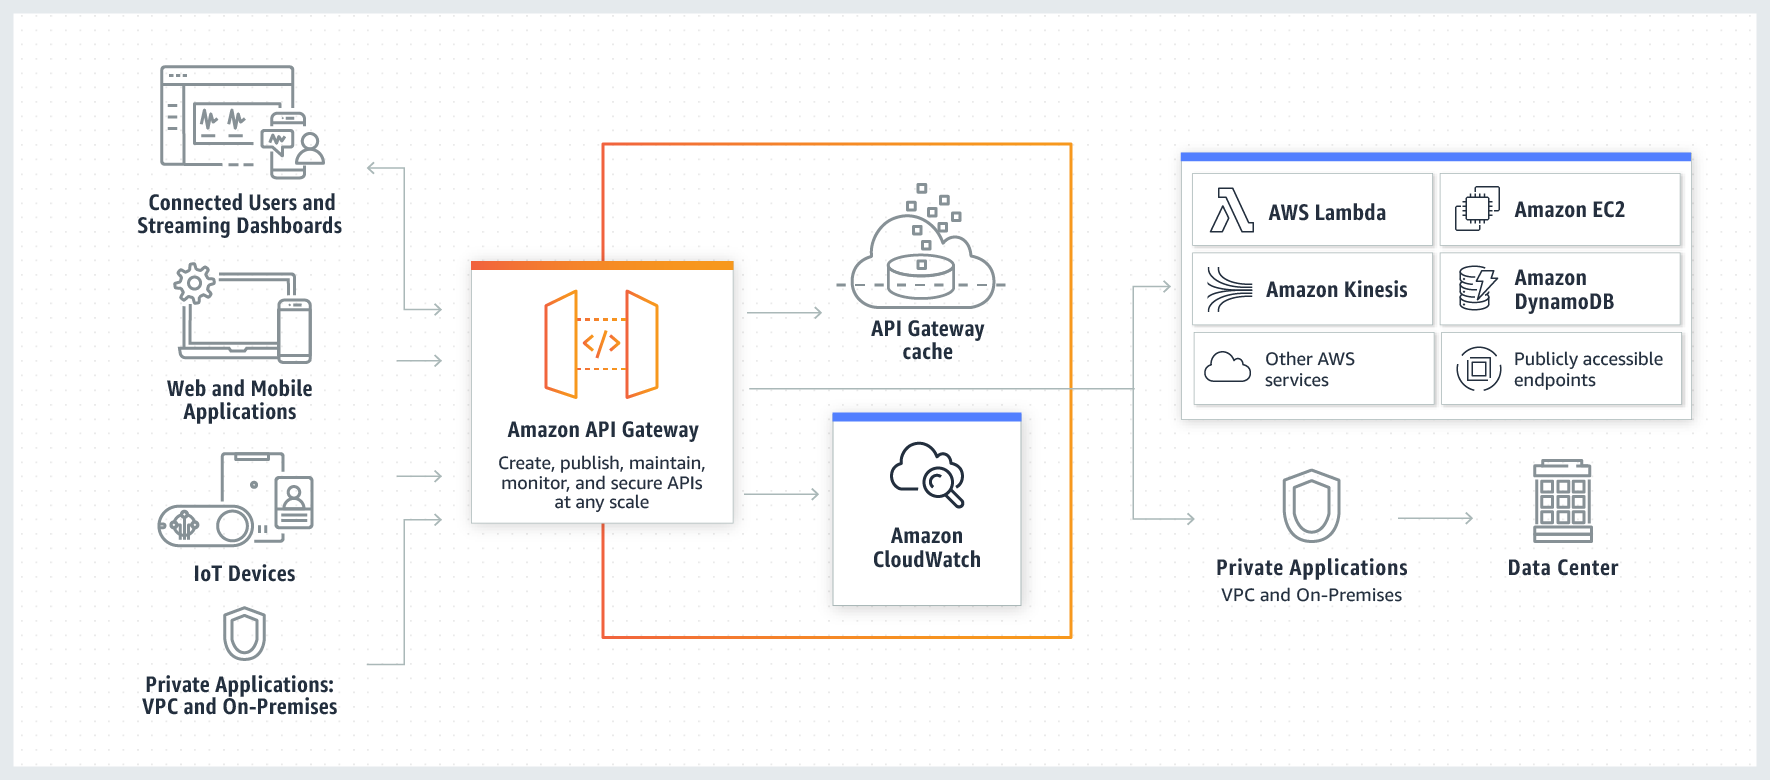
\includegraphics[width=0.8\textwidth]{Figures/apigateway}
	       \decoRule
		\caption[API Gateway]{API Gateway}
	\label{fig:apigateway}
	\end{figure}

%----------------------------------------------------------------------------------------

\section{Amazon Dynamodb}
Amazon DynamoDB est une base de données NoSql de type clé-valeur et de documents, offrant des performances de latence de l’ordre de quelques millisecondes, quelle que soit l’échelle. Il s’agit d’une base
de données multi-région, multi-active et durable entièrement gérée, avec des systèmes intégrés de sécurité,
de sauvegarde, de restauration et de mise en cache en mémoire pour les applications à l’échelle d’Internet.
DynamoDB peut traiter plus de 10 mille milliards de demandes par jour et supporte des pics de 20 millions
de demandes par seconde.\\

La plupart des entreprises du monde qui connaissent la croissance la plus rapide, comme Lyft, Airbnb et
Redfin, ainsi que Samsung, Toyota et Capital One s’appuient sur la mise à l’échelle et les performances de
DynamoDB pour prendre en charge leurs charges de travail stratégiques.
Des centaines de milliers de clients AWS ont choisi DynamoDB comme base de données de clés-valeurs et
de documents pour leurs applications mobiles, Web, de jeux, de technologie publicitaire, IoT, etc. nécessitant un accès à faible latence aux données, quelle que soit l’échelle
\newpage
\section{CloudWatch}
Amazon CloudWatch est un service de surveillance et d'observabilité conçu pour les ingénieurs DevOps, les développeurs, les ingénieurs en fiabilité de sites (SRE) et les responsables informatiques. \\

CloudWatch collecte des données de surveillance et opérationnelles sous forme de journaux, de métriques et d'événements. Ensuite, il les visualise à l'aide de tableaux de bord automatisés pour vous permettre d’avoir une appréciation unifiée de vos ressources, applications et services AWS opérationnels sur AWS et sur site.
 \begin{figure}[H]
            \centering
                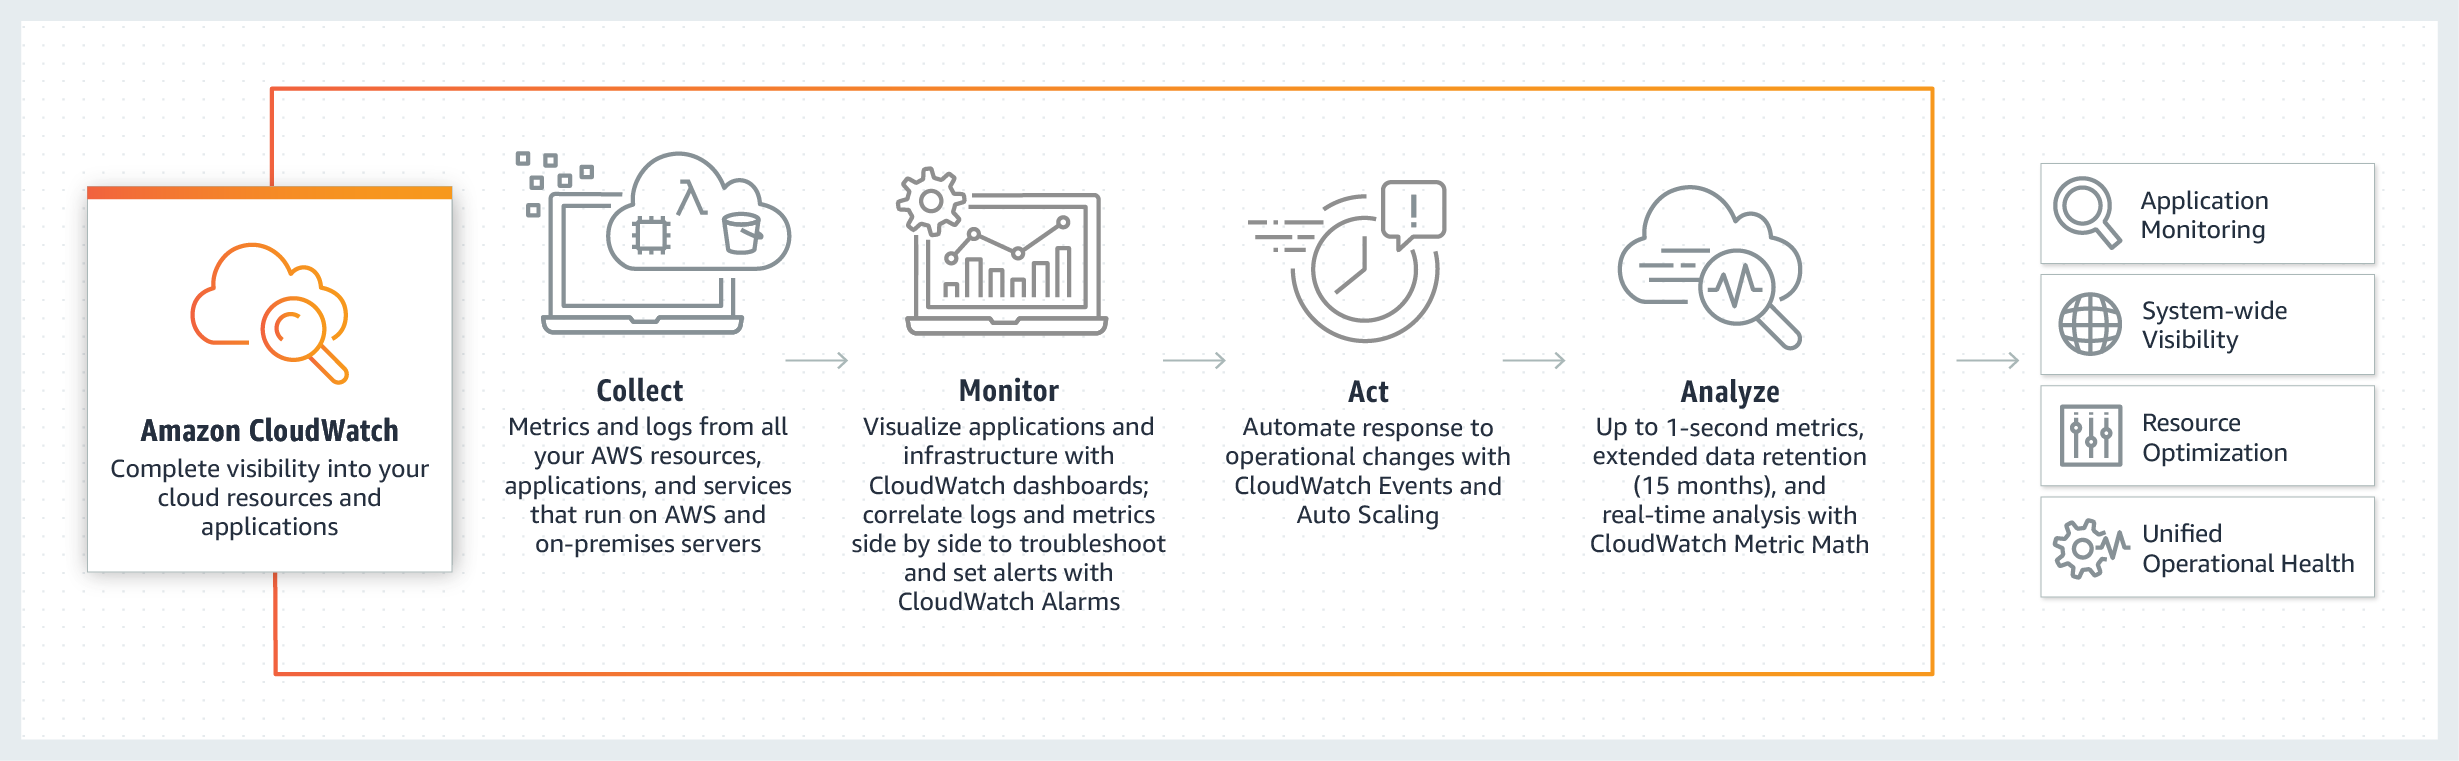
\includegraphics[width=0.8\textwidth]{Figures/cloudwatch}
	       \decoRule
		\caption[CloudWatch]{CloudWatch}
	\label{fig:CloudWatch}
	\end{figure}
\newpage
\section{Reflex}
ReFlex est un système de souscription automatisé modulaire. Il ne s'agit pas d'une application(service web) autonome, elle doit  être intégrée au paysage applicatif du client. Les composants ReFlex requis sont hébergés dans l'environnement du client. Chaque instance de Reflex est fournie avec une base de connaissance paramètrée en fonction des produits d'assurance du client(entreprise d'assurance).
Les principaux modules de Reflex sont:
\begin{list}{•}
\item \textbf{CEP:} Customer Experience Platform
\item
\item \textbf{RAS:} Risk Assessment Service
\item \textbf{DCS:} Document Creation Service 
\end{list}
\subsection{Scénario d'intégration CEP}
En incluant CEP dans le système, toutes les demandes adressées au composant RAS sont filtrées par le backend CEP. Et avant que l'évaluation des risques puisse être lancée, il doit y avoir une toute première étape d'initialisation pour initialiser l'utilisation du CEP. Cette étape comprend l'appel au service d'intégration, qui fait partie du backend CEP, pour créer un jeton Web JSON (JWT) qui sera transmis entre l'interface utilisateur et le backend pour identifier et autoriser l'utilisateur actuel.
 \begin{figure}[H]
            \centering
                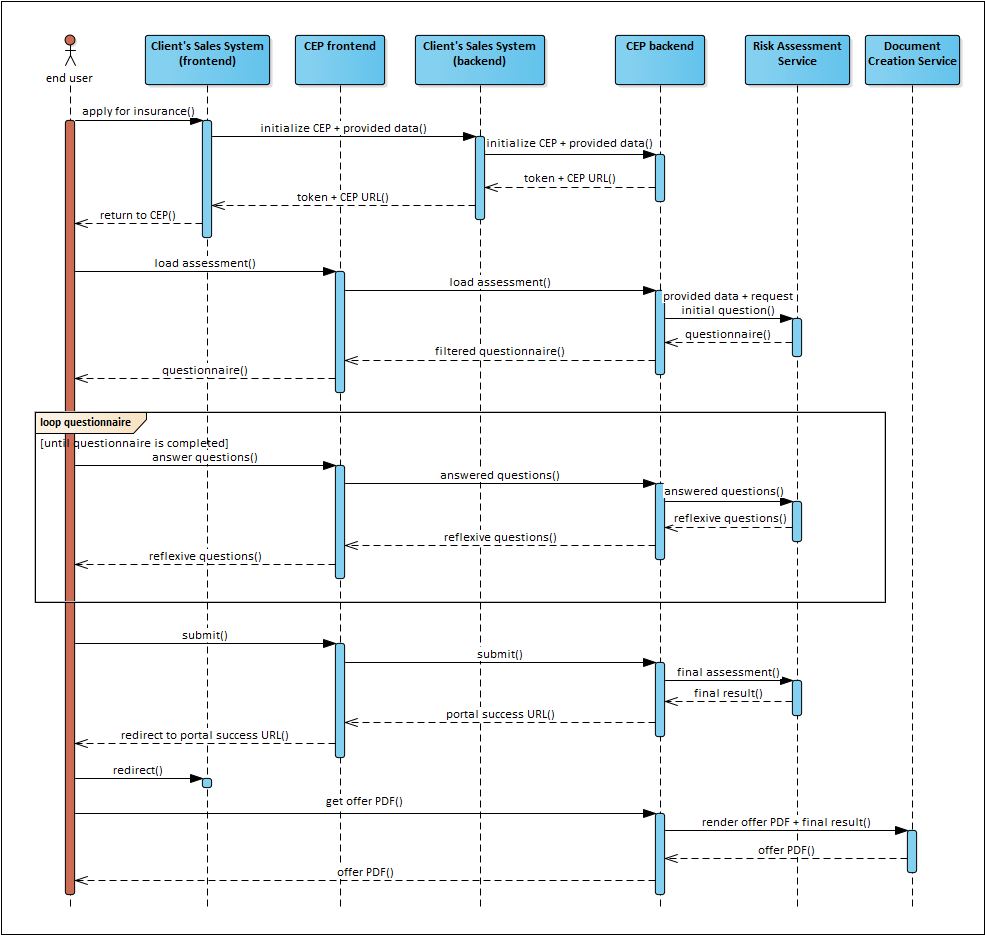
\includegraphics[width=0.8\textwidth]{Figures/cepreflex}
	       \decoRule
		\caption[Scénario d'intégration CEP]{Scénario d'intégration CEP}
\label{fig:Cep}
\end{figure}

% Chaptre 1

\chapter{Approche suivie et solution proposée} % Main chapter title

\label{Chaptre4} % For referencing the chapter elsewhere, use \ref{Chapter1} 

Dans cette section nous ferons une présentation détaillée des solutions que nous avions proposées par rapport à nos missions.

%----------------------------------------------------------------------------------------

% Define some commands to keep the formatting separated from the content 
%\newcommand{\keyword}[1]{\textbf{#1}}
%\newcommand{\tabhead}[1]{\textbf{#1}}
%\newcommand{\code}[1]{\texttt{#1}}
%\newcommand{\file}[1]{\texttt{\bfseries#1}}
%\newcommand{\option}[1]{\texttt{\itshape#1}}
%----------------------------------------------------------------------------------------

\section{Méthodologie de travail: Scrum avec Agile}
L’agrandissement de l’équipe tech et le besoin de fournir des livrables réguliers pour montrer l’évolution aux fonds d’investissement a nécessité la mise en place d’une nouvelle méthodologie de travail avec la méthode Agile Scrum.\\ \\ La méthode Agile est organisée en cycles de développements itératifs qui place le produit avant le projet. L’objectif n’est pas de terminer le projet mais de mettre en place un produit fini qui répond à toutes les exigences du client. Cette méthode part du principe que les besoins ne sont pas figés et peuvent évoluer avec le projet.\\ \\L’objectif final n’est pas défini au départ du projet mais des objectifs sont définis à court terme et fonctionne par étape. Une fois atteinte, un point est fait, les améliorations possibles sont mises en avant et l’étape suivante est définie en conséquence. Ce processus est ensuite répété jusqu’à l’obtention du produit final répondant à toutes les attentes. Avec ce fonctionnement, le client devient acteur du projet et peut être sollicité à chaque étape. Chaque étape doit durer 2-3 semaines maximum, comprenant des phases de test et le produit en sortie est incomplet mais doit être fonctionnel.\\ \\ La méthodologie Scrum reprend le cadre de travail Agile pour des projets plus complexes. Le projet est décomposé en «sprints» qui sont les étapes de développement. Afin de produire des livrables régulièrement et rapidement, nos sprints duraient une semaine.Une réunion est mise en place à chaque début de sprint afin de définir les objectifs de la semaine et leurs priorités. Durant toute la durée du sprint, une réunion quotidienne d’une durée de 30 minutes, « standup », a lieu, dans l’idée les participants restent debout pour éviter de s’éterniser. Chaque participant prend la parole afin de présenter son travail de la veille, valider les objectifs terminés et définir ceux du jour. Cette courte réunion doit servir à mettre en avant les points de blocage et synchroniser tous les membres de l’équipe. Le Scrum Master, chargé de vérifier le bon déroulement du sprint, doit valider avec l’équipe si les délais peuvent toujours être tenus et si le sprint est toujours réalisable dans son intégralité.\\ \\
Chaque fin de sprint comprend un point sur tous les objectifs validés ainsi qu’une démonstration du travail réalisé durant la semaine. Dans notre cas, un test de l’application est effectué afin d’obtenir des retours de tous les membres de l’équipe tech. Ces remarques seront ensuite prises en compte ou non dans le prochain sprint.
\subsection{Les principaux rôles de la méthodologie Scrum}
\begin{list}{•}
\item  \textbf{ Product Owner:} il est chargé de la vision du produit à réaliser et de définir les objectifs prioritaires.
\item
\item  \textbf{ Scrum Master:}membre de l’équipe chargé de vérifier la bonne application de la méthodologie de travail, il anime généralement les réunions quotidiennes. Ce rôle n’est pas figé et peut passer d’un membre à l’autre au sein de l’équipe.
\item  \textbf{ L’équipe de développement :}équipe chargée de réaliser les objectifs définis dans le sprint et se composant généralement de profil différent
\end{list}  
\newpage
\section{Les différentes missions et solutions}
\subsection{Mission 1:Etude de faisabilité sur le déploiement d’une application Front-End dans un environnement AWS}
L’application frontend(web app flutter) de Gighamesh est hébergée sur Firebase, tandis que l’essentiel de
ses ressources se trouve dans le cloud d’Amazon. C’est dans le but d’unifier nos environnements cloud que
cette mission m’avait été confiée.
\subsubsection{Observations}
Les applications web Flutter sont  développées avec le langage de programmation Dart. Avant le déploiement d'une application Flutter un build est nécessaire, 
et le résultat de celui-ci est un ensembles des fichiers statiques( html, css, js, ...). Ce sont ces fichiers statiques qui sont déployés.
Pour résoudre  j’avais exploré deux possibilités:
\subsubsection{Solutions}
\subparagraph{Solution1: L’utilisation de S3 comme repos de d'hébergement}
La solution ici consiste à créer un repos S3, de le rendre public, afin de pouvoir accepter tous les trafics.
De configurer Code Pipeline pour les besoins de CI/CD avec Github, De configurer Cloudfront pour la
gestion du trafic et Route 54 pour le routage.
 \begin{figure}[H]
            \centering
                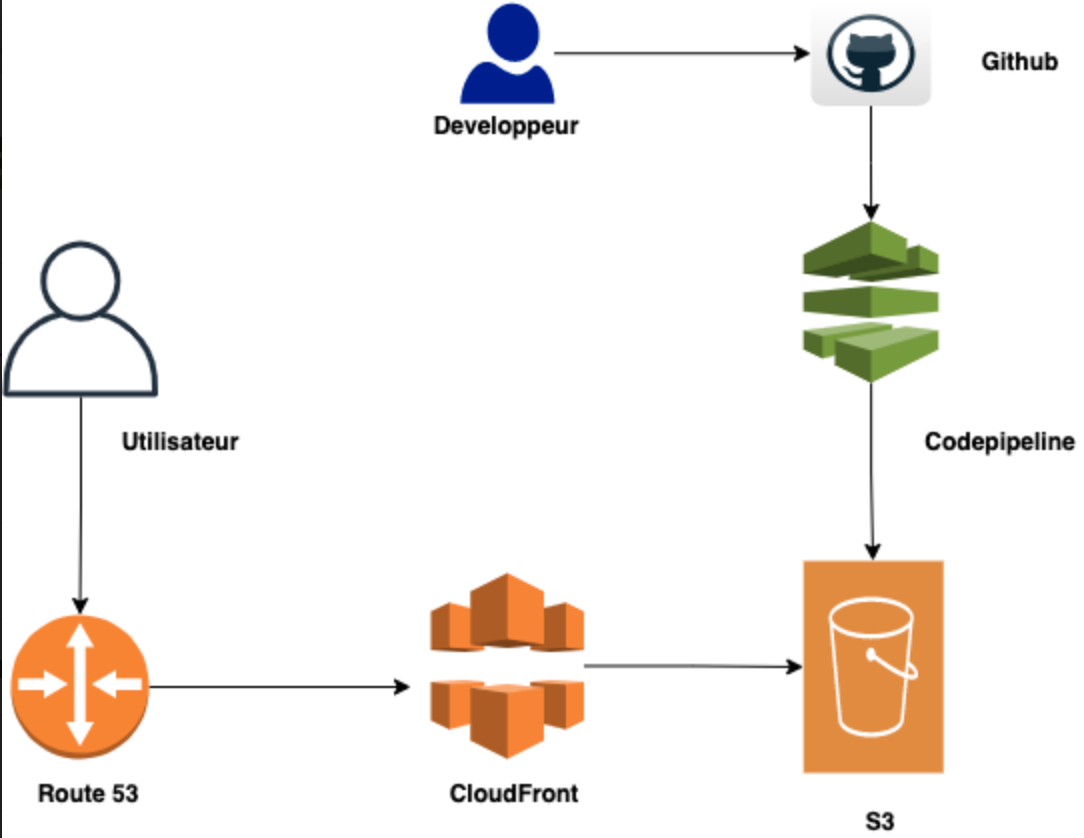
\includegraphics[width=0.8\textwidth]{Figures/S3}
	       \decoRule
		\caption[Solution à base de S3]{Solution à base de S3}
	\label{fig:S3}
	\end{figure}
\newpage
\subparagraph{Solution2: L’utilisation d’Amplify comme comme repos d'hébergement}
Cette solution consiste à utiliser le service d’hébergement qu’offre Amplify et son système de CI/CD en
l’associant au système de versioning: Github. J'avais utilisé CloudFront pour la gestion du trafic et Route 54
pour le routage.
NB: C’est la solution 2 qui avait été retenue. Celle-ci est simple et plus adaptée.
 \begin{figure}[H]
            \centering
                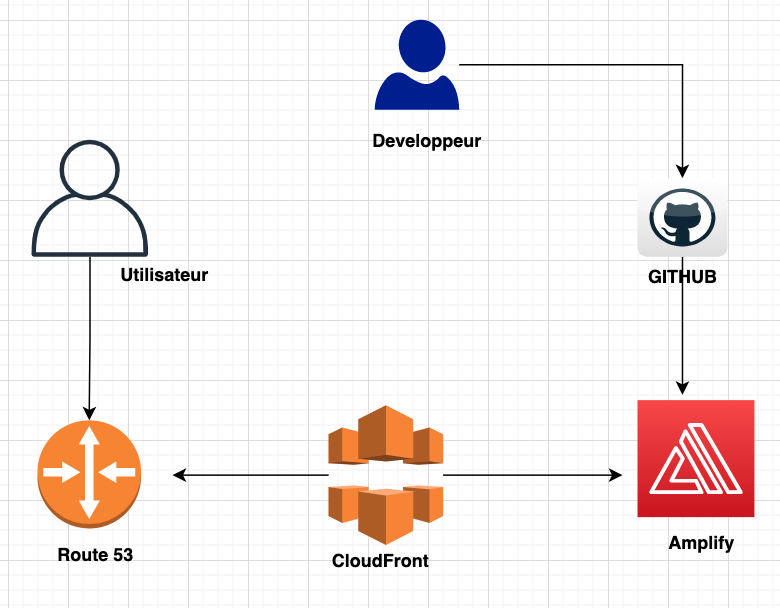
\includegraphics[width=0.8\textwidth]{Figures/amplify}
	       \decoRule
		\caption[Solution à base d'Amplify]{Solution à base d'Amplify}
	\label{fig:Amplify}
	\end{figure}
	
\subsection{Mission 2:Le déploiement et l’intégration du service web (Reflex) dans le parcours de souscription}
La souscription au produit d’assurance Assurly est subdivisée en trois parcours: P1, P2, et P3. Un utilisateur ne peut se
retrouver que dans un seul parcours en fonction des données fournies. Si un utilisateur se retrouve dans le
parcours P3 un questionnaire plus complexe est nécessaire, c’est à cet instant qu’intervient Reflex.
\newpage
\subsubsection{Solutions}
%Reflex est composé de trois modules de base: CEP pour frontend, DOCS pour la gestion des rapports et
%RAS qui constitue le cœur du système Reflex.
%La procédure de déploiement consiste mettre à jour le repos Github qui contient les fichiers nécessaires à la
%construction de notre container, à se connecter à notre EC2, à puller les fichiers du repos Github depuis un
%répertoire de notre EC2 puis à construire et déployer notre container avec la commande docker-compose.
\subsubsection{Pipeline de déploiement}
Quand nous recevons de notre partenaire des mises à jour des modules Reflex , nous les déployons(push) sur un repos Github. Notre repos Github est connecté à notre docker hub; ce qui déclenche automatiquement la construction et le déploiement(push) de l'image de notre conteneur sur docker hub. Pour déployer Reflex sur notre EC2: Il suffit soit de récupérer(pull) le contenu du repos Github puis construire l'image et déployer le conteneur ou de récupérer(pull) l'image de docker hub puis déployer le conteneur. La figure ci-dessous illustre le processus.  
 \begin{figure}[H]
            \centering
                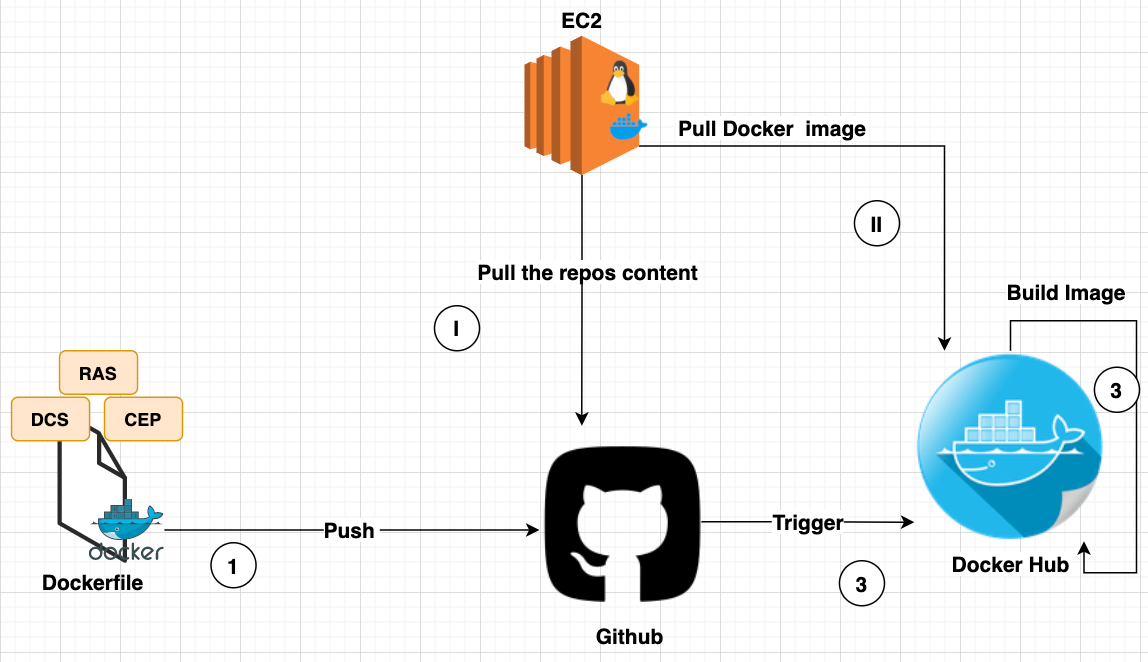
\includegraphics[width=0.8\textwidth]{Figures/pipeline1}
	       \decoRule
		\caption[Pipeline de déploiement de Reflex]{Pipeline de déploiement de Reflex}
	\label{fig:Pipeline de déploiement de Reflex}
\end{figure}

 \begin{figure}[H]
            \centering
                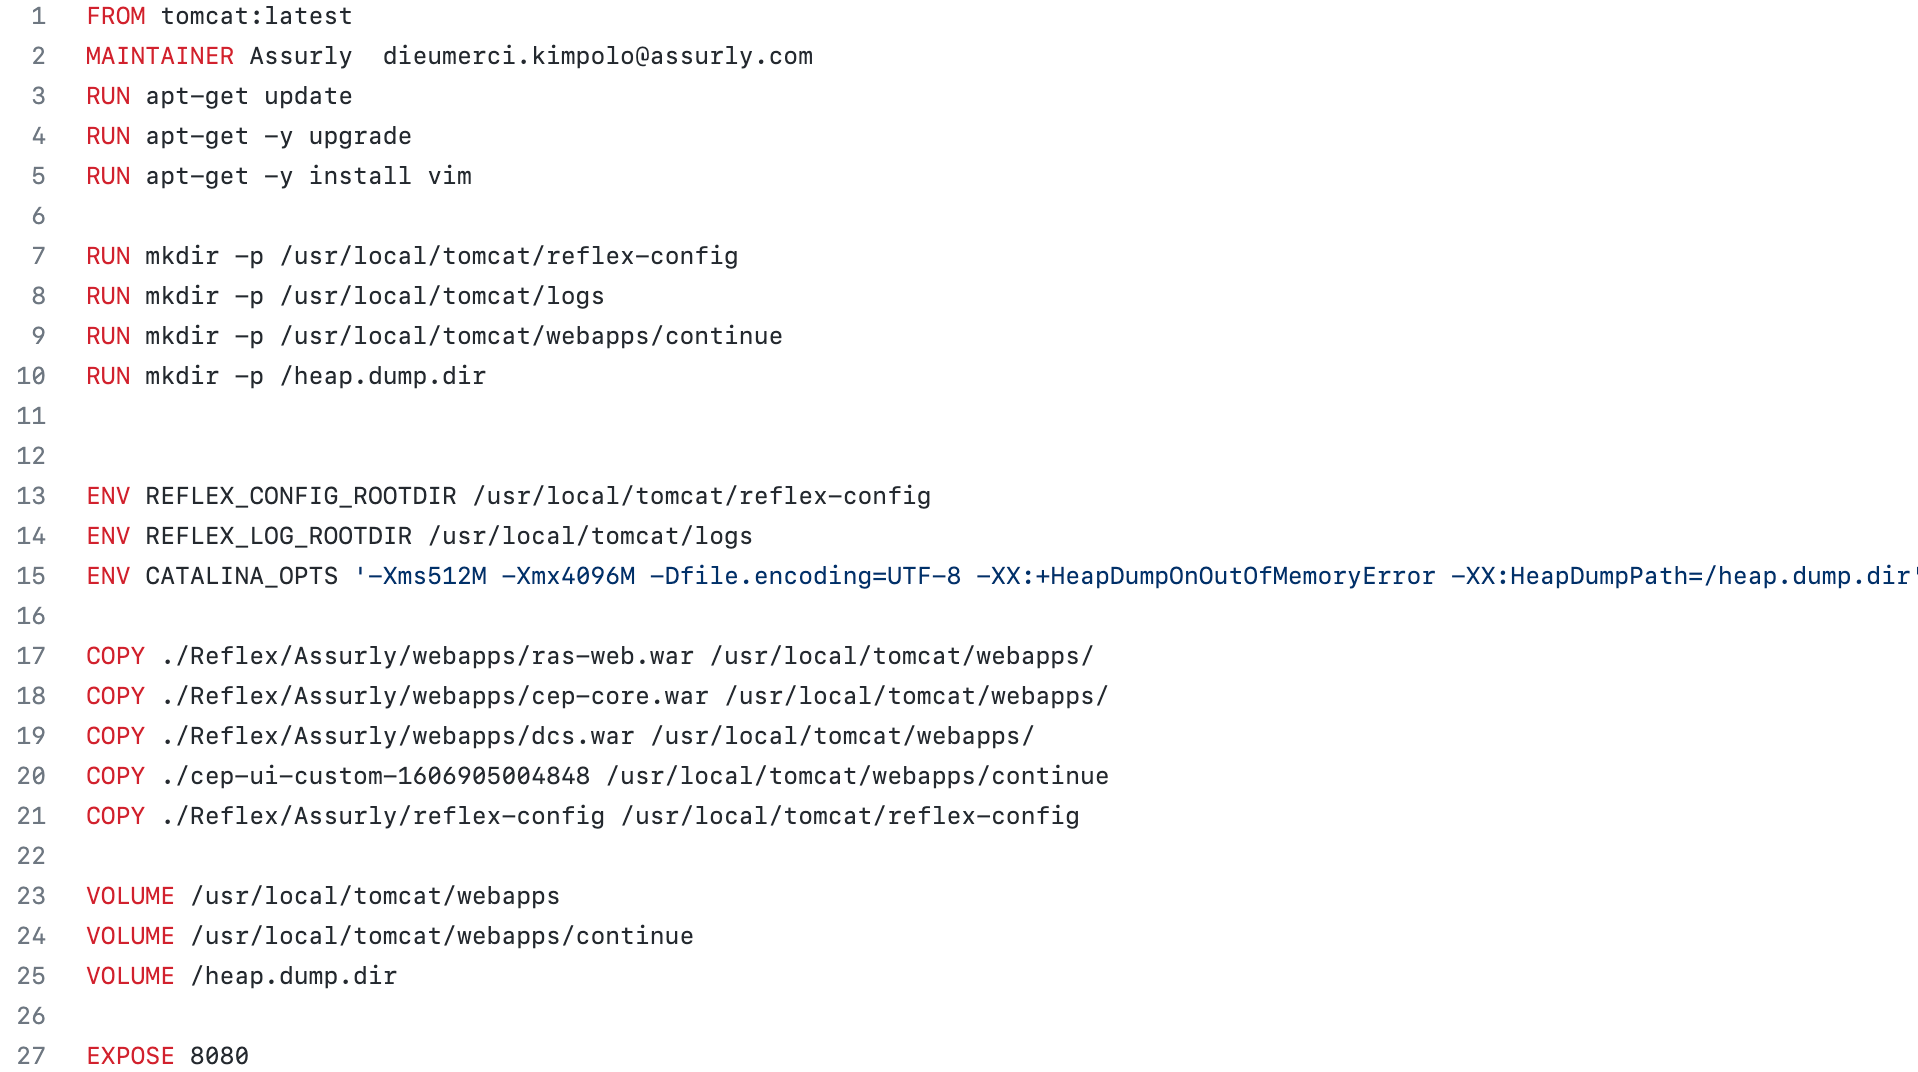
\includegraphics[width=0.8\textwidth]{Figures/dockerfile}
	       \decoRule
		\caption[Dockerfile de construction de l'image Reflex]{Dockerfile de construction de l'image Reflex}
	\label{fig:Dockerfile de construction de l'image Reflex}
\end{figure}
\newpage
\subsubsection{Diagramme de séquence intégration}
L'intégration de Reflex sur l'application web est différente de celle sur l'application mobile.

\textbf{Cas de l'application web}
Notre application web est embarquée dans une Iframe, et l'intégration de Reflex passe par une initialisation des cookies. Il nous était impossible d'initialiser les cookies d'un autre domaine depuis l'Iframe de notre application web. Pour palier ce problème nous avons développé une application intermédiaire hébergée sur le même server web que le moteur Reflex. Les utilisateurs en P3 qui passe par notre application web sont redirigés  sur  l'application web intermédiaire, pour soumettre leur questionnaire Reflex et sont redirigés sur l'application web depart à la fin du processus. Le BACKEND sur le diagramme de séquences ci-dessous représente notre infrastructure dans l'environnement AWS.
 \begin{figure}[H]
            \centering
                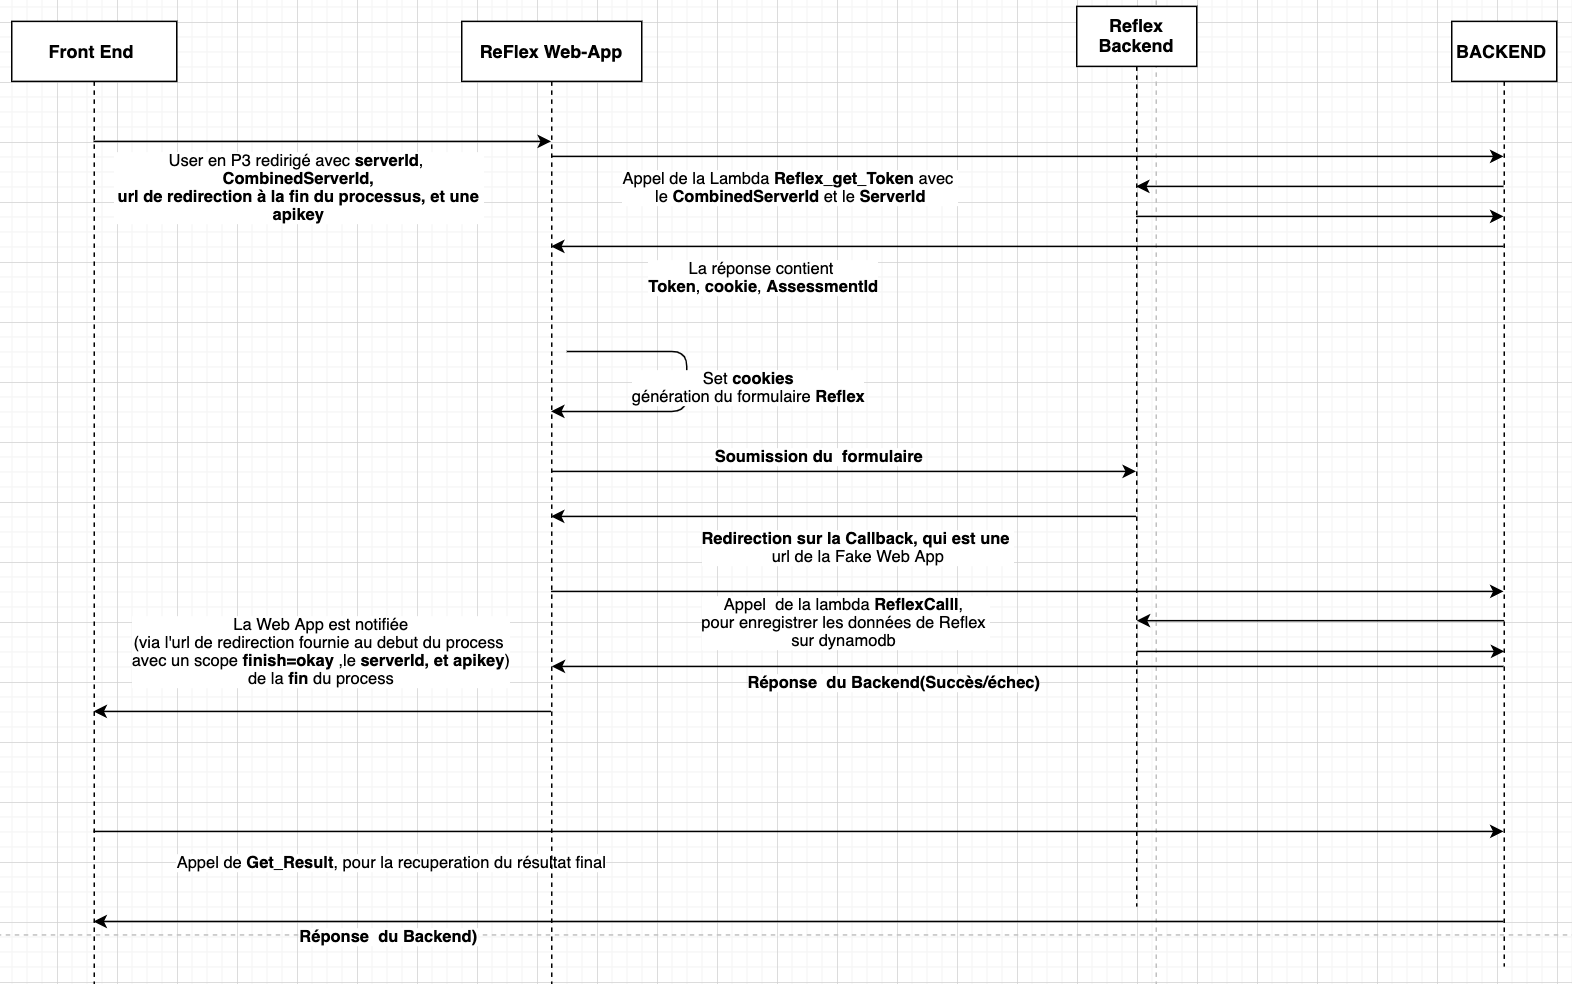
\includegraphics[width=0.8\textwidth]{Figures/reflexweb}
	       \decoRule
		\caption[Diagramme d'intégration de Reflex sur l'application web]{Diagramme d'intégration de Reflex sur l'application web}
	\label{fig:Diagramme d'intégration de Reflex sur l'application web}
\end{figure}

 \begin{figure}[H]
            \centering
                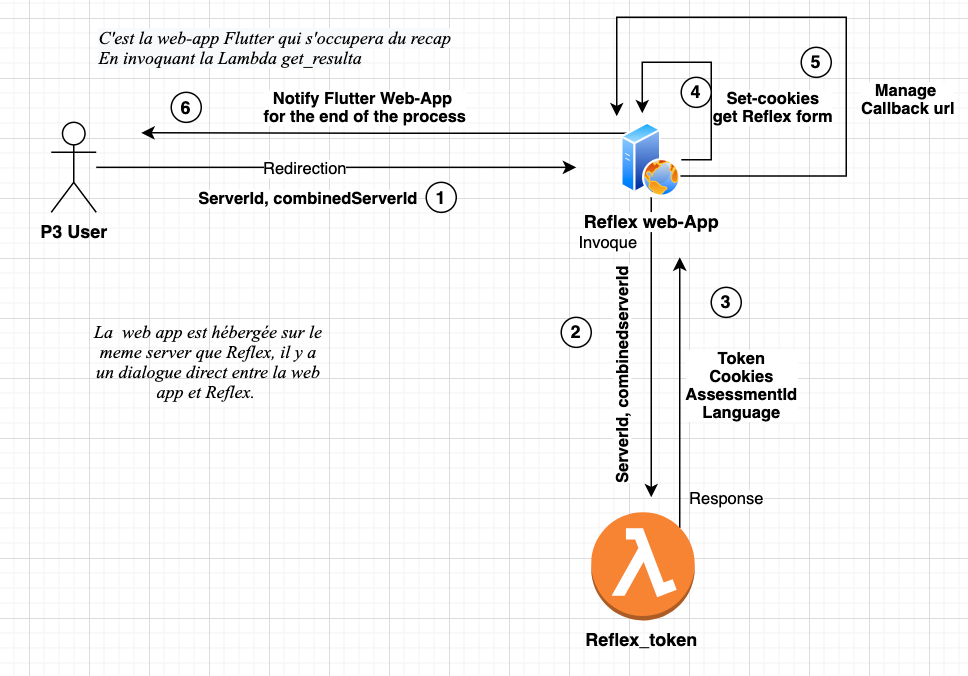
\includegraphics[width=0.6\textwidth]{Figures/reflexapp}
	       \decoRule
		\caption[Diagramme d'intégration de Reflex sur l'application web]{Diagramme d'intégration de Reflex sur l'application web}
	\label{fig:Diagramme d'intégration de Reflex sur l'application web}
\end{figure}
\newpage
\subsection{Mission 3: Etude de la sécurité actuelle d’accès aux API}
Les API sont devenues incontournables, il existe très peu ou presque pas de systèmes informatiques qui ne consomment et/ou ne fournissent des API. Dans la plus part des cas ou très souvent on est soit consommateur, soit fournisseur  ou les deux.\\ \\ Comme les applications classiques, les API n'échappent pas au problèmes de sécurité. Elles font face aux mêmes défis que les applications ordinaires. Elles sont vulnérables à plusieurs types  d'attaques comme: les attaques Dos et attaques par pollutions des paramètres http,...\\ La question de sécurité des API comme pour des applications ordinaires doit être pris en considération durant tout le cycle son développement: de sa conception à sa mise en production. \\Dans le cadre de mon étude je m'était focalisé sur les API de type Rest conçues et et déployées dans le cloud d'Amazon.\\ Dans l'environnement AWS les Backend des API sont protégés par le service API Gateway, et une très grande parties des protocoles de sécurité y sont implémentés.
\subsubsection{Rappel des principes de sécurité}
Un système sécurisé doit garantir les points suivants:
\begin{itemize}
\item \textbf{L'intégrité:} garantir que les données sont bien celles que l'on croit être
\item \textbf{La disponibilité:} maintenir le bon fonctionnement du système d'information
\item \textbf{La confidentialité:} rendre l'information inintelligible à d'autres personnes que les seuls acteurs d'une transaction
\end{itemize}
\subsubsection{La sécurité des API dans AWS}
Pour sécuriser une API dans l'environnement AWS il faut prendre en compte deux aspects suivants: 
\begin{enumerate}
\item Les contrôles d'accès 
\item L'authentification et les autorisations
\end{enumerate}
Il n'ya pas de choix à faire entre les contrôles d'accès et le système d'authentification \& d'autorisation, ils sont complémentaires.
\subsubsection{Les contrôles d'accès}
Les mécanismes suivants peuvent être utilisés pour effectuer d'autres tâches liées au contrôle de l'accès aux API dans AWS.
\begin{list}{•}
\item \textbf{Le partage des ressources cross-origin (CORS)}  permet de contrôler la façon dont votre API REST répond aux requêtes de ressources inter-domaines. 
\item
\item \textbf{Les certificats SSL côté client} peuvent être utilisés pour vérifier que les requêtes HTTP adressées à votre système backend proviennent d'API Gateway.
\item \textbf{AWS WAF} peut être utilisé pour protéger votre API d'API Gateway contre les menaces web courantes telles que l'injection SQL et les attaques XSS (cross-site 
scripting). 
\item \textbf{API Key} peut être utilisé pour gérer les quotas des appels de l'API
\item \textbf{API endpoints  ressorces policy} peut être utilisé pour refuser certains appels en fonction des adresse IP
\item \textbf{VPC endpoints policy } peut être utilisé pour gérer les endpoints accessibles seulement pour les adresse IP privées
\end{list}
 \begin{figure}[H]
            \centering
                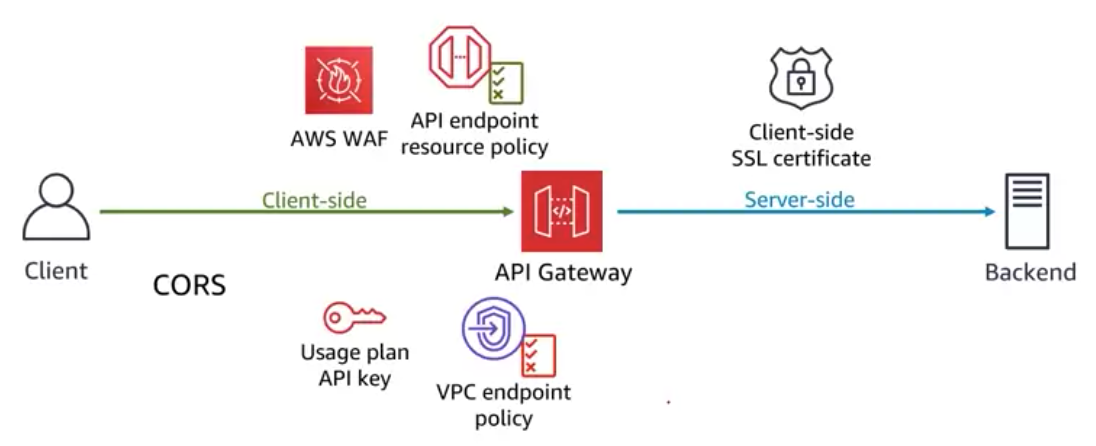
\includegraphics[width=0.8\textwidth]{Figures/controleaccess}
	       \decoRule
		\caption[Les contrôles d'accès]{Les contrôles d'accès}
	\label{fig:Les contrôles d'accès}
	\end{figure}
%\textbf{Password grant}
\subsubsection{Authentification et autorisations}
Le protocole de base de gestion des authentifications et des autorisations au niveau des API Rest est le protocole Oauth2, décrit dans la section état de l'art. Aws utilise essentiellement le service Cognito pour gérer les questions d'autorisation et d'authentification sur des API. Cognito dans son fonctionnement suit les principes de base du protocole Oauth2. 
%C'est Cognito que nous avons utilisé pour gérer les authentifications et les autorisations. 

\subsubsection{L'existent}

\textbf{Points positifs}\\
L'Api est accessible en https, les CORS et les contrôles d'accès par API Key sont implémentés sur l'API Gateway.
%\begin{enumerate}
%\item L'Api est accessible et https
%\item Implémentation des CORS et la gestion des API key sur l'API Gateway
%\end{enumerate}

\textbf{Points négatifs}\\
Le service Cognito est implémenté  mais consommé via de fonctions Lambda personnalisées, le service Cognito implémenté  et consommé via de fonctions Lambda personnalisées,
les données des utilisateurs filtrées avec des paramètres autres le token d'accès valide aussi un chiffrement  est implémenté sur les applications frontend en plus du ssl. 
%\begin{enumerate}
%\item Le service Cognito implémenté  et consommé via de fonctions Lambda personnalisées
%\item Les données des utilisateurs filtrées avec des paramètres autres le token d'accès valide
%\item Implémentation d'un chiffrement  supplémentaire en dehors du ssl
%\end{enumerate}

\subsubsection{Observations}
\begin{enumerate}
\item Cognito à la base ne peut supporter qu'un seul user pool (support de stockage des utilisateurs) sur une API
\item L'API  est  type Rest et déployé dans le cloud d'Amazon
\item Les utilisateurs  stockés dans  plusieurs users pool
\item L'API est consommée par des applications web et  mobiles
\end{enumerate}
Pour supporter plusieurs user pools sur nos API, nous avons développé un système d'autorisation personnalisé à base d'une Lambda. Dans notre implémentation nous avons exploré deux flows: l'implicit grant(en utilisant la web UI de Cognito) et password grant.

%L'intégrité : garantir que les données sont bien celles que l'on croit être. La disponibilité : maintenir le bon fonctionnement du système d'information. La confidentialité : rendre l'information inintelligible à d'autres personnes que les seuls acteurs d'une transaction.
\textbf{Implicit grant}
 \begin{figure}[H]
            \centering
                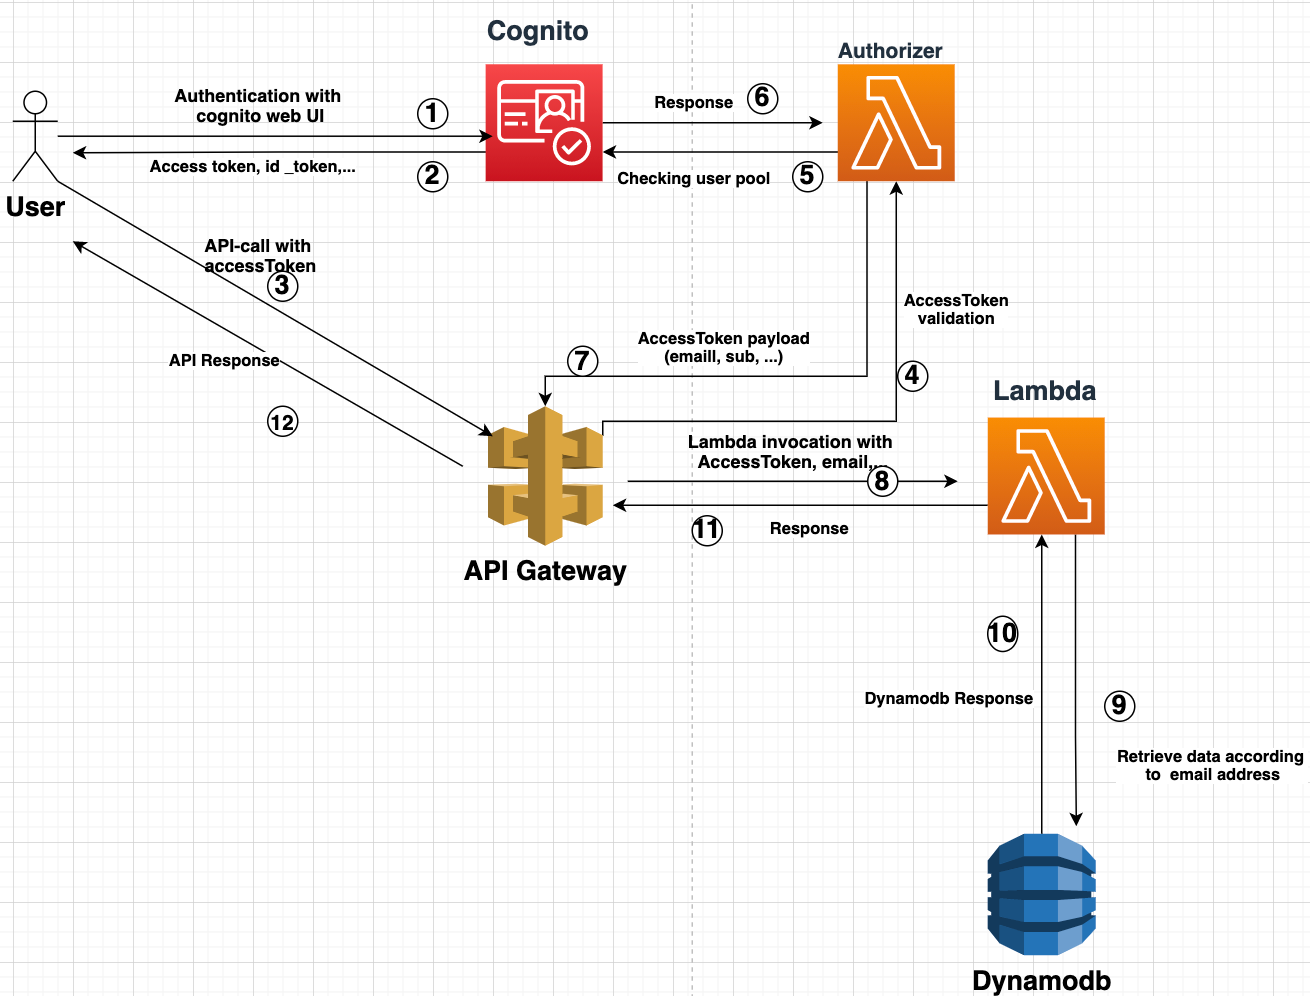
\includegraphics[width=0.8\textwidth]{Figures/securite}
	       \decoRule
		\caption[L'architecture du système de sécurité, Implicit grant]{L'architecture du système de sécurité, Implicit grant}
	\label{fig:L'architecture du système de sécurité, Implicit grant}
	\end{figure}
%\textbf{Password grant}
 
\newpage
\subsection{Mission 4(Mise en place d'un ETL d'intégration de données)}
Gigamesh disposait une quantité importantes des données stockées dans des fichiers txt; des données nécessaires pour effectuer des campagnes de marketing ciblées. Ma mission consistait à intégrer ces données dans une base de données sql pour pouvoir y effectuer facilement  des requêtes.

\subsubsection{Observations}
\begin{enumerate}
\item Tous les fichiers avaient la même structure
\item Le caractère | était utilisé comme séparateur des colonnes
\item Les libellés des colonnes étaient de fois des phrases
\item Les données n'étaient pas typées
\end{enumerate}
\subsubsection{Solution}
Pour résoudre le problème j'avais mise en place un \textbf{ETL}, qui récupère les données brutes(fichiers txt) de leur support de stockage, les transforme avec un \textbf{script Python} et les stocke dans base de données Mysql dans l'environnement AWS via le service Aurora. 

 \begin{figure}[H]
            \centering
                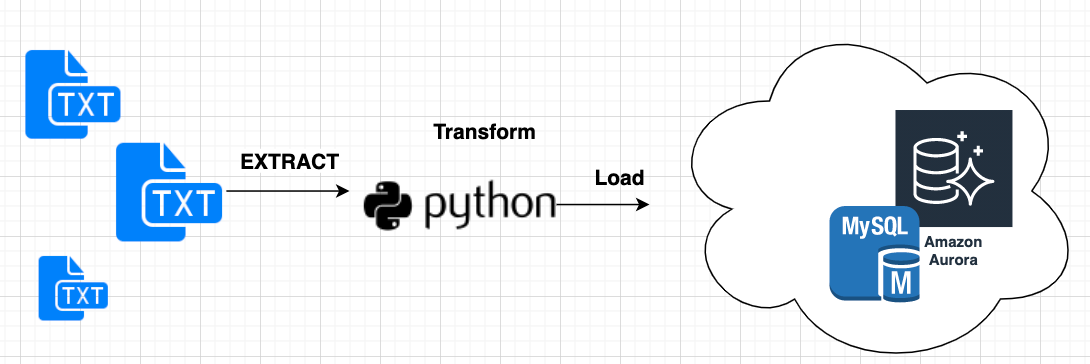
\includegraphics[width=0.8\textwidth]{Figures/etls}
	       \decoRule
		\caption[Etl d'intégration de données]{Etl d'intégration de données}
	\label{fig:etl}
	\end{figure}
La partie de transformation de mon ETL m'avait servi à la création de la table où sont stockées les données et à leur typage. 
 \begin{figure}[H]
            \centering
                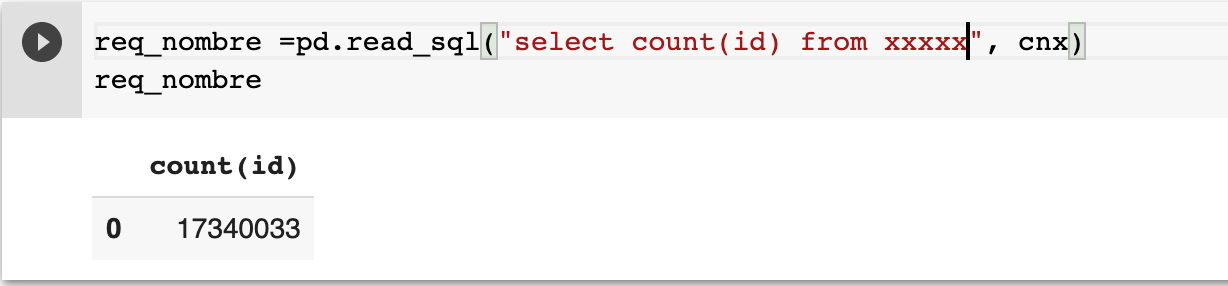
\includegraphics[width=0.8\textwidth]{Figures/nombre}
	       \decoRule
		\caption[La taille de la table où sont stockées nos données]{La taille de la table où sont stockées nos données}
	\label{fig:La taille de la table où sont stockées nos données}
	\end{figure}
 
%\include{Chapters/Chapter5} 

%----------------------------------------------------------------------------------------
%	THESIS CONTENT - APPENDICES
%----------------------------------------------------------------------------------------

\appendix % Cue to tell LaTeX that the following "chapters" are Appendices

% Include the appendices of the thesis as separate files from the Appendices folder
% Uncomment the lines as you write the Appendices

% Appendix A

\chapter{Frequently Asked Questions} % Main appendix title

\label{AppendixA} % For referencing this appendix elsewhere, use \ref{AppendixA}

\section{How do I change the colors of links?}

The color of links can be changed to your liking using:

{\small\verb!\hypersetup{urlcolor=red}!}, or

{\small\verb!\hypersetup{citecolor=green}!}, or

{\small\verb!\hypersetup{allcolor=blue}!}.

\noindent If you want to completely hide the links, you can use:

{\small\verb!\hypersetup{allcolors=.}!}, or even better: 

{\small\verb!\hypersetup{hidelinks}!}.

\noindent If you want to have obvious links in the PDF but not the printed text, use:

{\small\verb!\hypersetup{colorlinks=false}!}.

%\include{Appendices/AppendixB}
%\include{Appendices/AppendixC}

%----------------------------------------------------------------------------------------
%	BIBLIOGRAPHY
%----------------------------------------------------------------------------------------

\printbibliography[heading=bibintoc]

%----------------------------------------------------------------------------------------

\end{document}  
